%Dies ist die Hauptseite des Dokumentes. Es werden u. a. alle Kapitel,
%Einstellung im Header eingebunden.  Veränderungen müssen in folgenden Dateien
%vorgenommen werden:
      %- config.tex
      %- einzelne Kapitel (evtl. erweitern)

\input{common/layout.tex}          % Diese Datei enthält alle
                                          % Layouteinstellungen
\newcommand{\dokumentTitel}{Technischer Entwurf}
% Definition von globalen Parametern, die derzeit auf der Titelseite und in der
% Kopfzeile verwendet werden. Der in <> gesetzte Text ist zu verändern.

\newcommand{\praktikumTitel}{<Titel des Praktikums>}
\newcommand{\projektTitel}{<Titel des Teilprojektes>}
\newcommand{\institut}{
	<Name des Instituts>\\
	<Name des Institutsleiters>\\
	<Straße und Hausnummer>\\
	<Postleitzahl und Ort>\\
}
\newcommand{\institutsLogo}{common/ISF_Logo.pdf}
\newcommand{\betreuer}{<Name>}

%------Beginn des Gesamtdokumentes----------------------------------------------
\begin{document}

%------Eingebundene Seiten, Verzeichnisse bzw. Kapitel--------------------------
\include{common/titelseite}                      % Titelseite


\tableofcontents                          % Inhaltsverzeichnis wird automatisch
                                          % generiert
\listoffigures                            % ebenso das Abbildungsverzeichnis

%----Kapitel des Feinentwurfs, die mit Inhalt zu füllen sind--------------------
%!TEX root = ../TechnischerEntwurf.tex

\chapter{Einleitung}
Dieses Dokument dient dazu, einen tiefer gehenden Überblick über den internen Ablauf der zu entwickelnden Software zu bieten. Es werden zuerst die wichtigsten Funktionen einzeln beschrieben, wobei Sequenzdiagramme zu Hilfe genommen werden. Danach wird der Aufbau der Komponenten beschrieben, sowie deren Verteilung gezeigt und am Ende die Datenverwaltung näher beleuchtet. \\
Ziel ist es, dass ein Entwickler nach dem Lesen dieses Dokuments die Software nachentwickeln könnte.

\begin{figure}[h]
\includegraphics[width=1.0\textwidth]{figures/statechart_game.pdf}
\caption{Zustandsdiagramm zum oberflächlichen Spielablauf}
\label{state_game}
\end{figure}


Um eine Verständnisgrundlage zu schaffen ist in Abbildung 1.1 die allgemeine Men\"uf\"uhrung in einem Zustandsdiadramm dargestellt. 


Nach dem Einloggen gelangt man in das Main Menu. Von dort aus gelangt man in die drei Spielmodi (Story, Trivia, Homework), die Einstellungen, das Profil und in die Ranglisten.

Der Story Mode hat wiederum eine eigene Übersicht, Laboratory genannt. Von hier aus kann der User sich seine aktuellen Playerstatistiken im Charakter Sheet ansehen, kann sich in der Scrollcollection um die Herstellung von Potions und Enchantments k\"ummern, diese danach in seinen Belt einf\"ugen um sich im Anschluss dem Minispiel zu widmen. Im Minispiel werden dem User verschiedene Hindernisse vorgesetzt, die es zu überwinden gilt. Scheitert der User, so gelangt er in den Game Over Screen, in dem ihm angezeigt wird wie viele Lofi-Coins (die Spiel-Währung) und welche Scrolls er in dieser Runde eingesammelt hat. Nach Bestätigung befindet sich der User zurück im Laboratory.

Der Trivia-Mode stellt einen SQL-Trainer dar. Entscheidet der User sich dafür diesen zu verwenden, gelangt er in einen Screen, in dem er sich für einen Schwierigkeitsgrad entscheiden muss. Hat der User dies getan, erhält er eine, dem ausgewählten Schwierigkeitsgrad entsprechende, Aufgabe und kann diese lösen.

Der Homework-Mode funktioniert auf die gleiche Weise wie der Trivia-Mode, lediglich die Auswahl des Schwierigkeitsgrads entf\"allt in diesem Fall.
Die Funktion soll den Hausaufgaben-Ablauf der Vorlesung RDB1 unterstützen.

In den Rankings werden die Spieler nach verschiedenen Kriterien in Ranglisten sortiert. Darüber ist es auch möglich, durch die Eingabe des Benutzernamens, nach anderen Spielern zu suchen und sich deren Profil anzeigen zu lassen.
Das eigene Profil ist über das Main Menu zu erreichen und einsehbar. Selbiges gilt für die Spieleinstellungen.  



\section{Projektdetails}

Die Anzahl an Lofi-Coins, sowie die Anzahl an Scrolls, die der User pro Tag einsammeln kann, werden beschr\"ankt.
Dies soll verhindern, dass der User hauptsächlich oder ausschließlich das Minispiel spielt, was dem Zweck der Anwendung, nämlich dem Üben von SQL entgegenwirkt. Auf der anderen Seite soll so der Spieler zum Wiederkommen animiert werden.

Des Weiteren wurde im Pflichtenheft erwähnt, dass Spieler sich durch Aufgabenerstellung ins Spiel mit einbringen können. Um dabei jedoch eine gewisse Qualität gewährleisten zu k\"onnen, wird es nur beförderten Nutzern möglich sein, eigene Aufgaben zu erstellen. Wie ein User befördert wird, wird über die Spielzeit oder über Leistungen im Spiel geregelt.  




%\chapter{Einleitung}

%Hier erfolgt eine kurze Darstellung von Aufbau und Ziel dieses Dokuments.

%Hier ist die Arbeitsweise des Systems anhand von Aktivitätsdiagrammen 
%und/oder Statecharts darzustellen und kurz verbal beschreiben.



%Beispiele:
%\begin{itemize}
%\item Bei einem Spiel könnte der Ablauf des Spiels als Aktivitätsdiagramm dargestellt werden.
%\item In einen Web-System könnten die vom Nutzer sichtbaren Seiten als Zustände im Statechart modelliert werden.
%\end{itemize}

%\begin{figure}[ht]
%\centering
%\includegraphics[width=0.7\textwidth]{figures/activity}
%\caption{Ein beispielhaftes Aktivitätsdiagramm}
%\label{activity}
%\end{figure}

%Quelle der Abbildung \ref{activity}: http://www.uml-diagrams.org/

%\textbf{Hinweis zu den Templates:}\\
%Dieses Template enthält Hinweise und Beispiele, die selbstverständlich zu entfernen sind.
% Angaben in <...> sind mit dem entsprechendem Text zu füllen.
%Die Grafiken in diesem Dokument sind nur Beispiele und sind keine Vektorgrafiken. 

%\textbf{Aufgabe des Technischen Entwurfs:}\\
%Der Technische Entwurf dokumentiert die klassischen Entwurfsentscheidungen wie z.B. 
%die Verwendung bestimmter Bibliotheken oder Entwurfsmuster. Darüber hinaus bildet der 
%Technische Entwurf die Grundlage der Implementierung, d.h. anhand dieses Dokumentes 
%muss jeder Softwareentwickler in der Lage sein, das Produkt zu entwickeln.
% Es ist also auf Vollständigkeit der Dokumentation zu achten.\\
%\textbf{Kapitel die bereits im Fachentwurf bearbeitet wurden, müssen hier nicht erneut
% bearbeitet werden. Es sollten jedoch die Annotationen umgesetzt worden sein.
% Es sollen also Kapitel 3-5 und Kapitel 8-9 neu erarbeitet werden. Kapitel 10 soll an 
%dieses Dokument angepasst werden, wenn es notwendig ist.}

%\textbf{Dieses Kapitel kann aus dem Fachentwurf übernommen werden, 
%sollte jedoch die Bearbeitung der Annotationen beinhalten.}

%\section{Projektdetails}

%Besonders interessante oder komplizierte Sachverhalte sollen hier noch weiter vertieft werden.
% Auch hier sollen wieder Aktivitätsdiagrame und Statecharts verwendet werden.

%Beispiele:
%\begin{itemize}
%\item Bei einem Spiel könnten komplizierte Regeln dargestellt werden.
%\item In einen Web-System könnte bestimmte Workflows als Aktivitätsdiagramm dargestellt werden.
%\end{itemize}

%Es kann pro Sachverhalt ein Abschnitt hinzugefügt werden.


%!TEX root = ../Fachentwurf.tex

\chapter{Analyse der Produktfunktionen}\label{chap:analyse}
Im Folgenden werden die im Pflichtenheft benannten Funktionen näher beschrieben und erkl\"art. Dabei wird davon ausgegangen, dass der User sich in dem Interface befindet, in dem er die erklärte Funktion initiieren kann.

Desweiteren ist zu erkennen, dass, jedes mal wenn das Back-End nach der Registration oder dem Login aktiv wird, es zuerst einen \glqq checkSession()\grqq -Methodenaufruf startet. Dies ist die Überprüfung des Back-Ends, ob es selbst den User kennt, ob er die gebrauchten Rechte für die Aktion hat und ob die Aktion auch auf die zum User gehörigen Daten ausgeführt wird.

\newpage
\section{Analyse von Funktionalität <F10>: <Nutzer registrieren>}
\begin{figure}[htb]
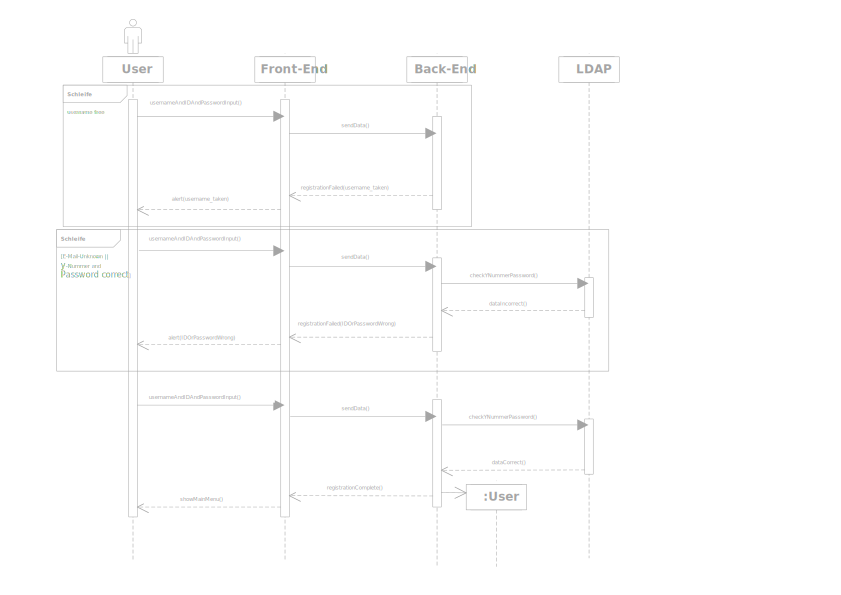
\includegraphics[width=1.3\textwidth]{figures/sequenz_F10.pdf}
\caption{Sequenzdiagramm zur Registrierung}
\label{sequence}
\end{figure}


\newpage
In Diagramm 2.1 wird der Vorgang der Registrierung beschrieben.

Dafür muss der User zuerst einen Username, eine E-Mail-Adresse oder seine y-Nummer (insgesamt ID genannt) und ein Passwort (im Falle einer y-Nummer das zur y-Nummer gehörende Passwort) angeben. Diese Eingaben werden dann an das Back-End übertragen. Hier wird zuerst geprüft ob der Username schon vergeben ist. Sollte das der Fall sein, wird dies dem User mitgeteilt und er muss einen neuen Username angeben.
Wenn der Username noch nicht vergeben war, wird, sollte die ID eine E-Mail-Adresse sein, geprüft, ob diese schon vorhanden ist. Wenn die ID eine y-Nummer ist wird diese inklusive des eingegebenen Passworts an das \glqq LADP\grqq geschickt und dort überprüft. Sollte der jeweils zutreffende Schritt fehlschlagen, muss der User seine Eingaben ändern beziehungsweise korrigieren und der Prozess beginnt von vorn.

Sollte der Ablauf erfolgreich verlaufen sein, erstellt das Back-End ein neues User-Objekt, speichert dies in seiner Datenbank und gibt die Rückmeldung, dass die Registrierung erfolgreich verlaufen ist und der User wird in das Hauptmenü weitergeleitet.
%==================================================================

\newpage
\section{Analyse von Funktionalität <F20>: <Nutzer anmelden>}
\begin{figure}[h]
\centering
\includegraphics[width=1.3\textwidth]{figures/sequenz_F20.pdf}
\caption{Sequenzdiagramm zum Login}
\label{sequence}
\end{figure}
Das Diagramm 2.2 beschreibt den Login-Vorgang. 

Hierbei muss der User die von ihm registrierte ID (siehe <F10>) und sein Passwort angeben. Diese werden, je nach Typ der ID, dann entweder mit der eigenen Datenbank verglichen, oder, sollte die ID eine y-Nummer sein, an das \glqq LDAP\grqq geschickt und dort überprüft.
Sollten die eingegeben Daten nicht korrekt sein, wir dies dem User mitgeteilt und er bekommt die Möglichkeit seine Eingaben zu korrigieren. Sind die Daten korrekt wird der User in das Hauptmenü weitergeleitet.
%==================================================================

\newpage
\section{Analyse von Funktionalität <F30>: <Nutzer abmelden>}
\begin{figure}[h]
\centering
\includegraphics[width=1.4\textwidth]{figures/sequenz_F30.pdf}
\caption{Sequenzdiagramm zum Login}
\label{sequence}
\end{figure}
Das Diagramm 2.3 beschreibt den Ablauf des Ausloggens.

Entscheidet sich der User sich auszuloggen, wir diese Information an das Back-End gesendet. Dieses beendet die Session des Users. Ist das geschehen wird eine Benachrichtigung an das Front-End gesendet und der User wird zurück zum Login-Screen geleitet.
%==================================================================

\newpage
\section{Analyse von Funktionalität <F40>: <Profil einsehen>}
\begin{figure}[h]
\centering
\includegraphics[width=1.3\textwidth]{figures/sequenz_F40.pdf}
\caption{Sequenzdiagramm zur Darstellung der Profilübersicht}
\label{sequence}
\end{figure}
Das Diagramm 2.4 zeigt was passiert, wenn man sich das eigene Userprofil anzeigen lassen möchte.

Um das Profil des Users anzuzeigen werden zuerst die Userdaten vom Back-End angefordert. Das Back-End lädt dann die Profildaten aus den Userdaten und schickt diese zurück an das Front-End. Dort werden sie für den User einsehbar im Profil-Interface angezeigt.

%==================================================================

\newpage
\section{Analyse von Funktionalität <F60>: <Passwort ändern>}
\begin{figure}[h]
\centering
\includegraphics[width=1.3\textwidth]{figures/sequenz_F60.pdf}
\caption{Sequenzdiagramm zum Ändern des Passworts}
\label{sequence}
\end{figure}
Das Diagramm 2.5 beschreibt das Ändern des Passwortes.

Das Ändern des Passwortes steht nur nicht-studentischen Nutzern zur Verfügung.
Entscheidet sich der Nutzer, sein Passwort zu ändern, kann er dies mit einem Klick auf den Change Password Button tun. Zuerst muss er sein altes Passwort eingeben und im Anschluss kann er ein neues Password erstellen. Dies muss danach noch einmal bestätigen werden und wenn alles erfolgreich war, wird das geänderte Passwort an das Back-End geschickt und dort in den Nutzerdaten vermerkt. Sollte während des Vorgangs etwas schief gehen, bleibt das alte Passwort bestehen und der User wird darüber in Kenntnis gesetzt.
%==================================================================

\newpage
\section{Analyse von Funktionalität <F70>: <Avatar ändern>} 
\begin{figure}[h]
\centering
\includegraphics[width=1.3\textwidth]{figures/sequenz_F70.pdf}
\caption{Sequenzdiagramm zum Ändern des Avatars}
\label{sequence}
\end{figure}
Das Diagramm 2.6 beschreibt das Ändern des Avatars.

Klickt der User auf den Change Avatar Button, werden ihm alle seine verfügbaren Avatare angezeigt und er kann sich für einen entscheiden. Hat er dies getan wird die Änderung der Einstellung vermerkt, ans Back-End geschickt, dort gespeichert und dann, wieder zurück im Front-End, aktualisiert angezeigt.
%==================================================================

\newpage
\section{Analyse von Funktionalität <F80>: <Benutzer löschen>} 
\begin{figure}[h]
\centering
\includegraphics[width=1.3\textwidth]{figures/sequenz_F80.pdf}
\caption{Sequenzdiagramm zum Löschen des Benutzers}
\label{sequence}
\end{figure}
Diagramm 2.7 zeigt, was passiert, wenn der User seinen Account löschen möchte.

Möchte der User sein Profil löschen, kann er dies im Settings-Interface tun, was dem entsprechend erst geladen werden muss. Wenn der User nun den Delete User Button drückt, wird der User erst noch einmal gefragt, ob er ein Profil wirklich löschen möchte. Beantwortet der User dies positiv geht eine Mitteilung an das Back-End, wo das Profil gelöscht wird und der User auf den Login-Screen geleitet wird wo es ihm frei steht, sich wieder zu registrieren.
%==================================================================

\newpage
\section{Analyse von Funktionalität <F90>: <Audioeinstellungen bearbeiten>}
\begin{figure}[h]
\centering
\includegraphics[width=1.3\textwidth]{figures/sequenz_F90.pdf}
\caption{Sequenzdiagramm zum Ändern der Audioeinstellungen}
\label{sequence}
\end{figure}
Diagramm 2.8 zeigt, was passiert, wenn der User seine Audio-Optionen ändert.

Zum Ändern der Audiofunktionen stehen Knöpfe bereit, die sowohl die Hintergrundmusik (\glqq Music\grqq) als auch die Soundeffekte, wie Sprungsounds und Klicksounds,  aus- beziehungsweise einstellen. Jegliche \"Anderung wird sofort ans Back-End gesendet, dort gespeichert und dann im Profil aktualisiert.
%==================================================================

\newpage
\section{Analyse von Funktionalität <F100>: <Spielstand zurücksetzen>}
\begin{figure}[h]
\centering
\includegraphics[width=1.3\textwidth]{figures/sequenz_F100.pdf}
\caption{Sequenzdiagramm zum Zurücksetzen des Spielstands}
\label{sequence}
\end{figure}
Diagramm 2.9 beschreibt das Zurücksetzen des Storyfortschrittes.

Der User kann per Knopfdruck seinen Story-Fortschritt zurücksetzen. Tut er dies, muss er vorher noch einmal seine Zustimmung zum Löschvorgang geben. Ist auch dies geschehen, wird die Anweisung zum Löschen des Storyfortschrittes des Users an das Back-End geschickt und dort ausgeführt.
%==================================================================

\newpage
\section{Analyse von Funktionalität <F110>: <Tutorial spielen>}
\begin{figure}[h]
\centering
\includegraphics[width=1.0\textwidth]{figures/sequenz_F110.pdf}
\caption{Sequenzdiagramm für das Tutorial}
\label{sequence}
\end{figure}
Diagramm 2.10 zeigt den Ablauf im Tutorial.

Wird das Tutorial gestartet, werden zuerst alle Tutorial-Texte vom Back-End angefordert. Diese werden dann, wenn benötigt, dem User angezeigt. Zuerst wird der User in den Dungeon geleitet. Dafür werden die Leveldaten vom Back-End geladen, sodass der User den Dungeon betreten und Spielen kann. Hierbei kann er Schriftrollen (\glqq Scrolls\grqq) und Münzen (\glqq Lofi-Coins\grqq) einsammeln, was jeweils sofort ans Back-End gesendet und dort im Story-Progress bzw. in den Profildaten gespeichert wird.
Scheitert der User an einer Hürde im Dungeon, bekommt er zuerst einen Game-Over-Screen angezeigt, auf dem zusehen ist, was er eingesammelt hat und wird zur\"uck in den Labor-Screen geleitet.
Dort wird er per Tutorial-Text zur Scrollcollection geleitet um sich dort für ein Trank-Rezept zu entscheiden. Ist dies getan, wird aus dem Back-Ende eine für das Rezept passende Aufgabe angefordert und dem User angezeigt. Für diese Aufgabe hat der User keine Versuchsbegrenzung. Die Eingaben des Users werden dabei immer an das Back-End gesendet und dort kontrolliert. Hat der User die Aufgabe richtig gelöst, erhält er eine Potion und kann diese danach im Dungeon verwenden.
%==================================================================

\newpage
\section{Analyse von Funktionalität <F120>: <Story spielen>}
\begin{figure}[h]
\centering
\includegraphics[width=1.0\textwidth]{figures/Aktivitaetsdiagramm.pdf}
\caption{Aktivitätsdiagramm für den Story Mode}
\label{sequence}
\end{figure}
Der Story-Mode besteht aus sich abwechselnden Teilen aus SQL-Trainer und Minispiel. Um dies  besser zu zeigen, ist in Abbildung 2.11  das Aktivitätsdiagramm für den Story Mode aus dem Pflichtenheft abgebildet.

Darin ist zusehen, dass man sich im Labor einen oder mehrere Tränke brauen kann (SQL-Trainer-Anteil) um diese dann im Dungeon zu verwenden (Minispiel-Anteil).
Um die beiden Teile für sich besser beschreiben zu können, sind diese in den folgenden zwei Funktionen aufgeführt.
%==================================================================

\newpage
\section{Analyse von Funktionalität <F130>: <SQL-Trainer spielen>}
\begin{figure}[h]
\centering
\includegraphics[width=1.3\textwidth]{figures/sequenz_F130.pdf}
\caption{Sequenzdiagramm für den SQL-Trainer}
\label{sequence}
\end{figure}


Der SQL-Trainer ist Teil der drei Spielmodi (Story, Trivia, Homework) und wird einmal, wie er im Trivia-Mode verwendet wird, erklärt. Die leichten Abweichungen der anderen Spielmodi werden im Anschluss erwähnt. Diese benötigen wenig bis gar keine weitere Erklärung, da sie nur einen oberflächlichen Unterschied machen.

Zuerst werden dem User f\"unf Schwierigkeitsgrade angezeigt aus denen der er wählen kann. Hat er sich für einen Schwierigkeitsgrad entschieden, wird dies dem Back-End mitgeteilt, was daraufhin eine, dem gewählten Schwierigkeitsgrad entsprechende, Aufgabe bereitstellt. Diese kann dann vom User gelöst werden. Die Eingaben werden dabei immer ans Back-End geschickt und dort auf Richtigkeit geprüft. 

Ist die Prüfung positiv verlaufen wird der User wieder zur Schwierigkeitsgrad-Auswahl weitergeleitet.


Abweichungen zum Story-Mode:\\
Es werden keine Schwierigkeitsgrade angezeigt, sondern schon eingesammelte Rezepte für Tränke. Diese beinhalten in ihrer Definition schon die Schwierigkeitsgrade für die daraus hervorgehenden Aufgaben.


Abweichungen zum Homework-Mode:\\
Beim Homework-Mode wird die Auswahl des Schwierigkeitsgrades in jeglicher Form übersprungen und der Aufgabentext wird direkt angezeigt.  
%==================================================================

\newpage
\section{Analyse von Funktionalität <F140>: <Minispiel spielen>}
\begin{figure}[h]
\centering
\includegraphics[width=1.3\textwidth]{figures/sequenz_F140.pdf}
\caption{Sequenzdiagramm für das Minigame}
\label{sequence}
\end{figure}
Die Abbildung 2.13 zeigt die Abläufe im Dungeon.

Im Minispiel bewegt sich die Figur stetig nach rechts. Der User kann springen, wodurch er verschiedene Hindernisse überwinden kann. Desweiteren kann der User Lofi-Coins und Scrolls einsammeln. Dies wird sofort im Back-End vermerkt und im Spielerprofil und im Storyprogress gespeichert. Dem User ist zudem möglich vorher erstellte Potions zu verwenden um deren Effekte zur Überwindung von Hindernissen zu nutzen.

%==================================================================

\section{Analyse von Funktionalität <F150>: <Hausaufgaben bearbeiten>}
Die Bearbeitung von Hausaufgaben funktioniert wie das Nutzen des SQL-Trainers. Genauere Erklärungen sind dort (F130) zufinden.
%==================================================================

\section{Analyse von Funktionalität <F160>: <Ranglisten einsehen>}
\begin{figure}[h]
\centering
\includegraphics[width=1.2\textwidth]{figures/sequenz_F160.pdf}
\caption{Sequenzdiagramm für die Ranglisten}
\label{sequence}
\end{figure}
In Abbildung 2.14 wir das Anzeigen der Ranglisten dargestellt.

Möchte der User die Ranglisten einsehen, wird eine Anfrage an das Back-End gesendet. Das Back-End stellt dann die Daten für die Ranglisten zusammen und sendet diese dann zurück ans Front-End wo diese dann für den User einsehbar präsentiert werden.
%==================================================================

\newpage
\section{Analyse von Funktionalität <F170>: <Spieler suchen>}
\begin{figure}[h]
\centering
\includegraphics[width=1.3\textwidth]{figures/sequenz_F170.pdf}
\caption{Sequenzdiagramm zum Suchen eines anderen Users}
\label{sequence}
\end{figure}
Im Diagramm 2.15 ist zu sehen, wie man nach einem anderen User suchen kann.

Um einen anderen User zu suchen wird ein Usersuche-Feld bereitgestellt. Der dort eingegebene Name wird an das Back-End weitergeleitet und dort in der Userdatenbank gesucht und wenn er existiert wird dessen Profil aus der Datenbank geladen dem suchenden User angezeigt. Ist der Name in der Datenbank nicht zu finden, wird dem suchenden User das mitgeteilt.
%================================================================== 

\newpage
\section{Analyse von Funktionalität <F180>: <Hausaufgabenergebnisse einsehen>}
\begin{figure}[h]
\centering
\includegraphics[width=1.3\textwidth]{figures/sequenz_F180.pdf}
\caption{Sequenzdiagramm zum einsehen der eigenen Hausaufgabenergebnisse}
\label{sequence}
\end{figure}
Abbildung 2.16 beschreibt das Anzeige der Hausaufgabenergebnisse.

Nach dem Einloggen in das Admintool werden die Hausaufgabenergebnisse eines nicht-beförderten Users direkt aus der Datenbank geladen und angezeigt.
Ist der User schon \glqq befördert\grqq muss er erst noch auf den Show Homework Results Button drücken.
%==================================================================

\newpage
\section{Analyse von Funktionalität <F190>: <Benutzer befördern>}
\begin{figure}[h]
\centering
\includegraphics[width=1.3\textwidth]{figures/sequenz_F190.pdf}
\caption{Sequenzdiagramm zum Befördern eines Users}
\label{sequence}
\end{figure}
Abbildung 2.17 beschreibt das Befördern eines Benutzers.

Zuerst wird für den Admin die Userdatenbank angzeigt. Hier kann er entweder manuell oder per Suchfunktion nach einem User suchen und per Knopfdruck befördern, was dann im Back-End in den jeweiligen Userdaten registriert und gespeichert wird. 

Der Ablauf, einen User Adminrechte (<F200>) zu geben, gleicht dem des User Bef\"orderns.
%==================================================================

\newpage
\section{Analyse von Funktionalität <F210>: <Eine Trivia-Aufgabe erstellen>}
\begin{figure}[h]
\centering
\includegraphics[width=1.3\textwidth]{figures/sequenz_F210.pdf}
\caption{Sequenzdiagramm für das Erstellen von Aufgaben}
\label{sequence}
\end{figure}
Abbildung 2.18 beschreibt das Erstellen von eigenen Aufgaben.

Beförderte Nutzer können selber Aufgaben erstellen die später im Trivia Mode verwendet werden können.
Dafür steht im Admin-Tool ein Interface zur Verfügung in das ganz einfach alle zur Aufgabe gehörigen Daten einsammelt und dann ans Back-End sendet, welches die Aufgabe dann speichert. Sind nicht alle wichtigen Felder ausgefüllt, wird der User alarmiert und muss dies berichtigen damit dich Aufgabe gespeichert werden kann.
%==================================================================

\newpage
\section{Analyse von Funktionalität <F220>: <Benutzeraufgaben bewerten>}
\begin{figure}[h]
\centering
\includegraphics[width=1.3\textwidth]{figures/sequenz_F220.pdf}
\caption{Sequenzdiagramm zum bewerten User-erstellter Aufgaben.}
\label{sequence}
\end{figure}
Abbildung 2.19 zeigt den Ablauf, wie man eine User-erstellte Aufgabe bewertet.

In der Liste aller User-erstellten Aufgaben kann sich der User Aufgaben aussuchen, diese Ansehen und sie bewerten und kommentieren. Die Bewertung wird dann im Back-End für die Aufgabe registriert und gespeichert. 
%==================================================================

\newpage
\section{Analyse von Funktionalität <F230>: <Hausaufgaben erstellen>}

Die Erstellung von Hausaufgaben gleicht der User-seitigen Erstellung von Aufgaben, ist jedoch nur Administratoren zugänglich.

Der Unterschied zur normalen Aufgabenerstellung besteht darin, dass ein Aufgabenpaket erstellt wird. Dabei kann man entweder Aufgaben für das Paket neu erstellen, oder auf schon einmal erstellte Aufgaben, die in der Datenbank gespeichert sind, zugreifen. Diese Aufgabenpakete können dann noch mit zusätzlichen Parametern versehen werden, wie zum Beispiel einem Bearbeitungszeitraum oder einer Anzahl an Versuchen. 

%!TEX root = ../Systementwurf.tex

\chapter{Resultierende Softwarearchitektur}\label{chap:architektur}

Die \NewsGenie Systemarchitektur ist eine klassische Client-Server Architektur, wobei es sich um einen Thin-Client
und einen Fat-Server handelt. Sämtliche Rechenaufwändige Operationen werden dementsprechend auf dem \textit{Server} ausgeführt,
während der \textit{Client} die sprachbasierte Bedienung durch den User umsetzt. Allerdings werden kleinere und ressourcenarme  Sprachverarbeitungsdienste zum Zweck einer zeitlichen Performancesteigerung ebenfalls am \textit{Client}
realisiert. Diese beinhalten die Verarbeitung von Anfragen der einfachsten Art, in erster Linie einfache Navigationsbefehle, wie das Auswählen eines von mehreren vorgeschlagenen Nachrichtenartikeln. 
Die Kommunikation mit der \textit{Google-Speech-API} findet ebenfalls auf dem \textit{Client} statt.

Die Architektur des \textit{Servers} ist in vier Komponenten geteilt. Das Kernelement für die Datenspeicherung ist 
die mit Triplen realisierte \textit{Datenbank} und der \textit{Crawler}, welcher permanent die ausgewählten Nachrichtenseiten nach neuen Artikeln durchsucht, um diese dann speichern zu lassen. Aus der vom \textit{Client} empfangenen Useranfrage und den vorhandenen Artikeln in der \textit{Datenbank} eine relevante Antwort zu generieren ist Aufgabe des \textit{Query Processors}. 
Der \textit{Server} bietet darüber hinaus ein \textit{Web Interface} an, welches es dem User oder Administrator ermöglicht Benutzereinstellungen zu verändern.

Die Architektur des \textit{Query Processors} unterteilt sich in sechs weitere Komponenten. Herzstück ist der \textit{Query Handler}.
Diese Komponente steuert den Ablauf des \textit{Query Processors} und regelt das Zusammenspiel der anderen Komponenten. 
Die erste anzusteuernde Komponente ist \textit{Natural Language Processing}, welches die Satzstruktur der Useranfrage analysiert. Darauf aufbauend ist es im \textit{Analyzer} möglich die Intention der Nutzeranfrage zu bestimmen, wie z.B. Neuigkeiten im Bereich der Technologie zu finden, oder Informationen zu einer bestimmten Person zu nennen. 
Der \textit{Searcher} kann dementsprechend agieren und eine geeignete Anfrage an die Datenbank stellen. Im Falle einer Entitätsfrage, wie das erwähnte Fragen nach dem Alter einer Person, wird die \textit{Linked Open Data}-Komponente angesteuert, andernfalls die \textit{Datenbank}.
Die Informationen der Linked Open Data können durch die \textit{Linked Open Data} Komponente schnell und effizient abgefragt werden, um dementsprechende faktuale Anfragen beantworten zu können. 
Die bis hierhin entstandenen Ergebnisse des Prozesses werden daraufhin an die \textit{Result Processing} Komponente übermittelt.
Aufgabe dieser ist es, die Ergebnisse für die Sprachausgabe am \textit{Client} vorzubereiten, also den Ausgabestring zu generieren. Dazu zählt auch die Aufgabe durch Textbausteine für eine natürlich klingende und abwechslungsreiche Sprache zu sorgen.

\section{Komponentenspezifikation}

%In diesem Abschnitt wird die aus der Analyse der Produktfunktionen (\autoref{chap:analyse}) resultierende Komponentenstruktur zunächst überblickartig durch ein Komponentendiagramm beschrieben. Die Bezeichnungen und Anzahl der Komponenten
%muss natürlich konsistent sein mit der in \autoref{chap:analyse}!

%Die einzelnen Komponenten werden anschließend kurz beschrieben.

Die aus Abschnitt \ref{chap:analyse} resultierende Komponentenarchitektur ist in Abb.~\ref{fig:Komponenten} in Form eines Komponentendiagramms abgebildet. Die Komponente \textit{Query Processor} wird außerdem in Abb.~\ref{fig:Komponenten_QP} in ihre Unterkomponenten aufgeschlüsselt.

\begin{figure}
\centering
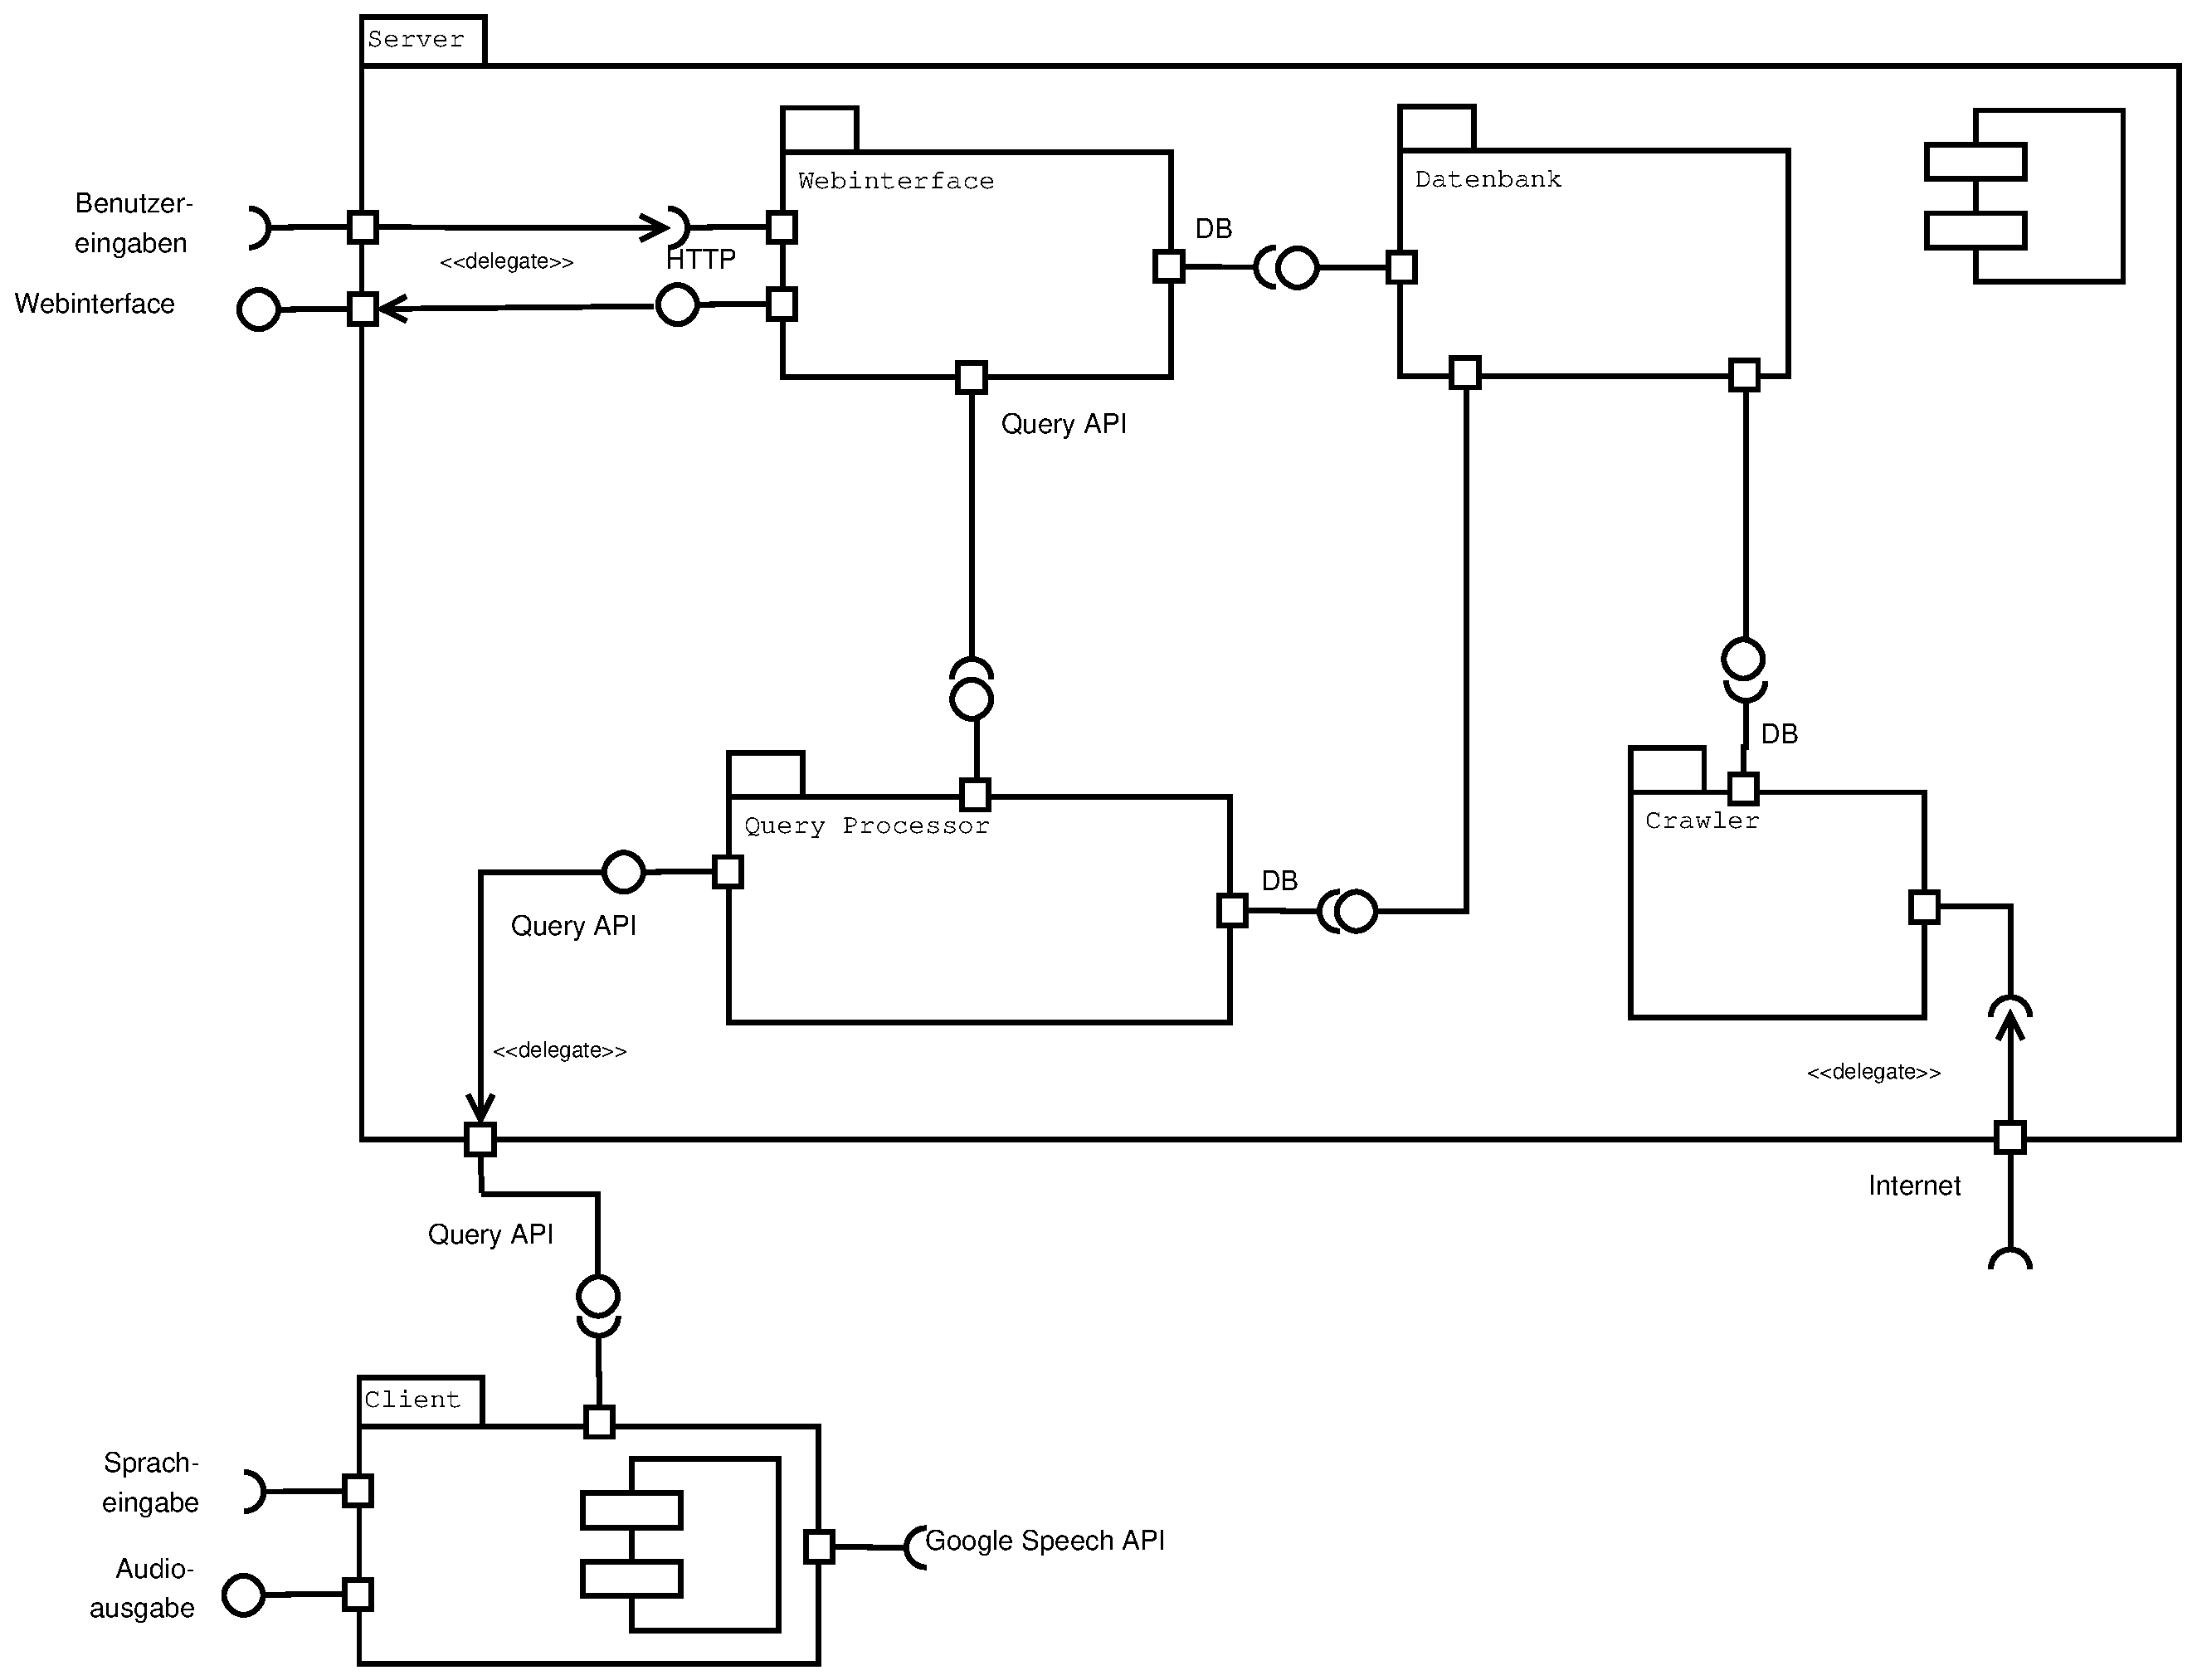
\includegraphics[width=1\linewidth]{Systementwurf/05_implementierungsentwurf/komponenten}
\caption{\textit{\NewsGenie Komponentendiagramm}}
\label{fig:Komponenten}
\end{figure}

\begin{figure}
\centering
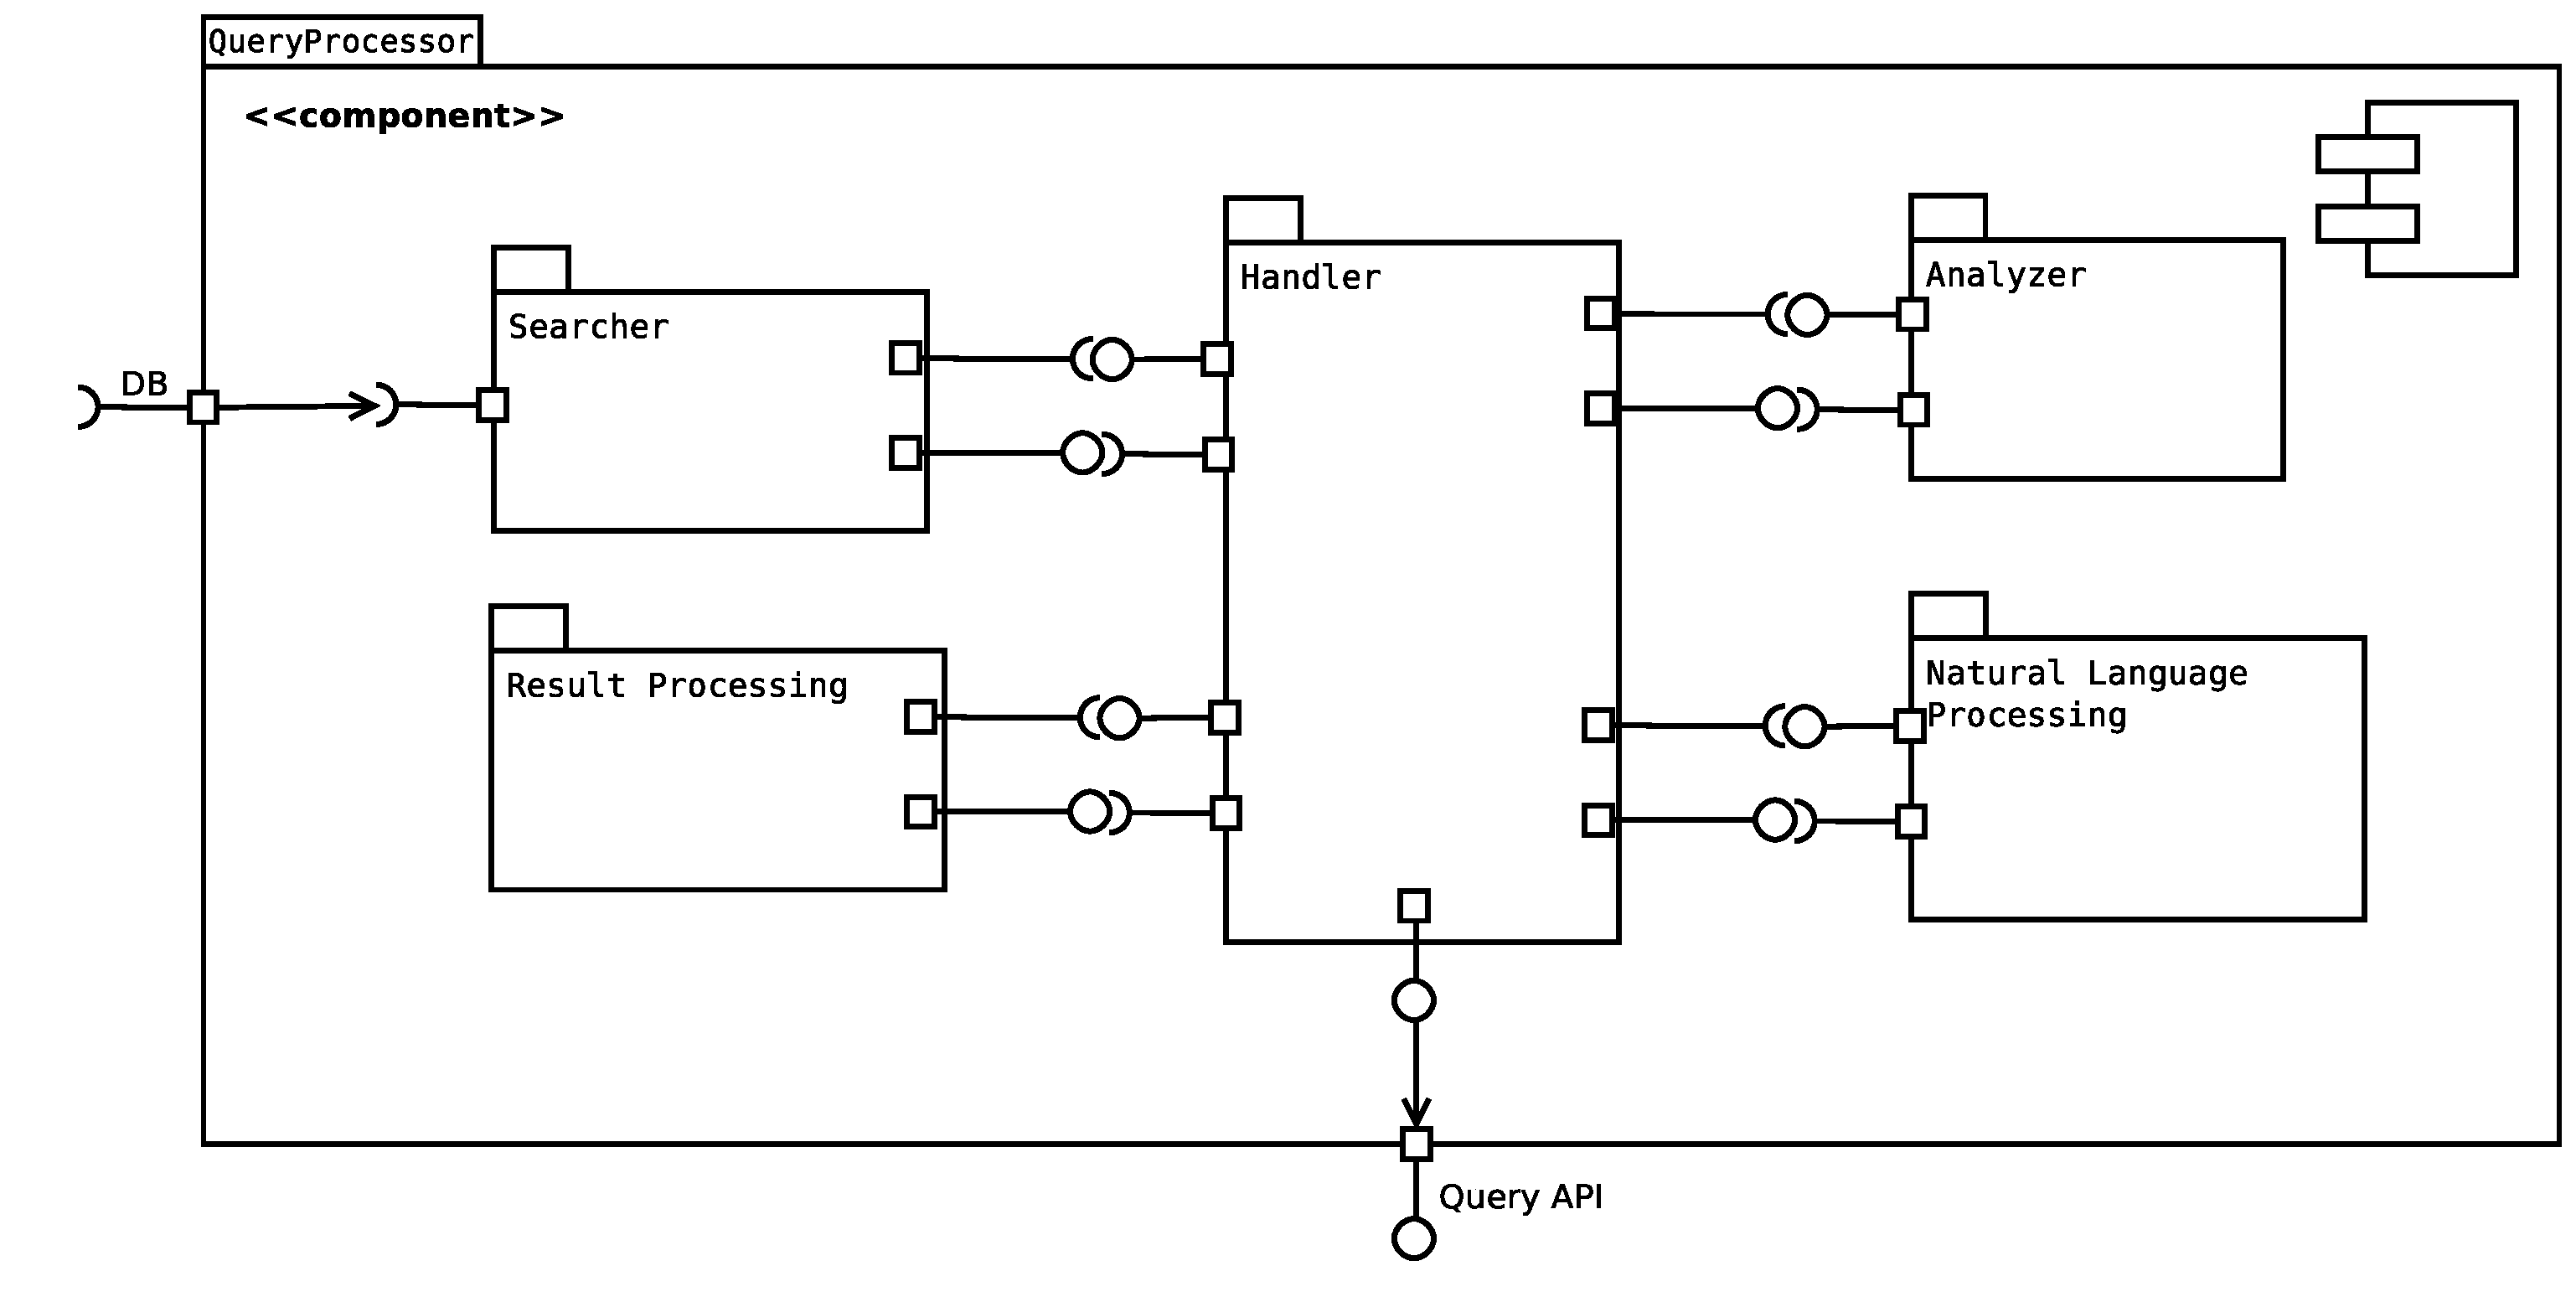
\includegraphics[width=1\textheight, angle=90]{Systementwurf/05_implementierungsentwurf/paket-queryprocessor}
\caption{\textit{\NewsGenie Komponentendiagramm - Query Processor}}
\label{fig:Komponenten_QP}
\end{figure}

\begin{component}{10}{Client}
Auf dem \textit{Client} werden die Hauptfunktionen der Sprach Ein- und Ausgabe realisiert. Der \textit{Client} ist somit die Hauptschnittstelle des Benutzers. Der Zugriff auf die \textit{Google Speech API} wird auf dem \textit{Client} realisiert. 
Die Komponente ist zusätzlich dazu in der Lage, auf simple Navigationsbefehle zu reagieren, ohne den \textit{Server} 
kontaktieren zu müssen.
\end{component}

\begin{component}{20}{Webinterface}
Das \textit{Web Interface} ist die zweite Schnittstelle für den Benutzer. Es stellt Konfigurations- und 
Administrationsfunktionen zur Verfügung, wie Nutzerregistrierung, Passwortmanagement, das Abonnement-Management
der Nachrichtenfeeds oder auch das Löschen von Nutzern.
\end{component}

\begin{component}{30}{Datenbank}
Realisiert die Speicherung der relevanten Daten über die User und die Nachrichtenartikel.
Die Speicherstruktur ist mit Tripeln implementiert.
\end{component}

\begin{component}{35}{Linked Open Data}
Komponente für den Zugriff auf die Linked Open Data. Sie liefert Informationen zu bestimmten
Entitätsfragen nach Personen oder Orten.
\end{component}

\begin{component}{40}{Crawler}
Der \textit{Crawler} liefert die Daten für die \textit{Datenbank}, indem er das Internet nach Nachrichtenartikeln
durchsucht, welche anschliessend gespeichert werden.
\end{component}

\begin{component}{50}{Query Processor}
Der \textit{Query Processor} verarbeitet die am \textit{Client}/\textit{Web Interface} gestellten Anfragen um die Intention
des Users zu erkennen und dementsprechend Anfragen an die \textit{Datenbank} zu stellen. Die Ergebnisse
werden an den \textit{Client} zurück gegeben.
Die Komponente besteht aus den Unterkomponenten \textit{Handler}, \textit{Natural Language Processing}, \textit{Analyzer}, \textit{Searcher}, \textit{Linked Open Data}, und \textit{Result-Processing}.
\end{component}

\begin{component}{60}{Handler}
Der \textit{Handler} steuert durch Aufrufe der anderen Komponenten den Ablauf im Query Processor. Sie ist die Komponente die von aussen angesteuert wird. 
\end{component}

\begin{component}{70}{Natural Language Processing}
Die als String eingehenden Anfragen werden auf ihre Satzstruktur analysiert. Es werden Subjekt, Objekt und Prädikat erkannt.
Darüber hinaus wird der Satz als Baumstruktur abgespeichert, was es ermöglicht Nebensätze und Hauptsätze zu erkennen. 
\end{component}

\begin{component}{80}{Analyzer}
Aufbauend auf \textit{Natural Language Processing} kann die Anfrage in dieser Komponente tiefer gehend analysiert werden. Sie bestimmt den Fragetyp, d.h. Entitätsfrage oder Nachrichtenanfrage, und kann somit die Intention des Users analysieren. 
\end{component}

\begin{component}{90}{Searcher}
Aufbauend auf den \textit{Analyzer} kann der \textit{Searcher} Datenbankanfragen stellen, um die passenden Ergebnisse zu bekommen.
Bei Entitätsfragen wird \textit{Linked Open Data} angesteuert, welche mit Daten aus der Linked Open Data antworten kann. 
\end{component}

\begin{component}{100}{Result Processing}
Im \textit{Result Processing} werden die Ergebnisse als String aufbereitet. Dabei werden variable Textbausteine verwendet um eine möglichst natürliche und flüssige Sprachausgabe zu gewährleisten.
\end{component}


\section{Schnittstellenspezifikation}

%Im Folgenden werden die einzelnen Schnittstellen der Komponenten aus der
%Komponentenspezifikation näher erläutert, d.h. die von Ihnen zur Verfügung
%gestellten Operationen werden dokumentiert. Die Tabelle ist dabei um so viele
%Zeilen zu erweitern, wie es Schnittstellen im Komponentendiagramm gibt. In der
%innen liegenden Aufteilung ist für jede Operation einer Schnittstelle eine
%Zeile einzufügen.  Reine Set- und Get-Aufrufe brauchen nicht aufgeführt zu
%werden (sollten auch möglichst nicht komponentenübergreifend auftauchen).

\textbf{Hinweis:}
Durch die Verwendung des Akka-Frameworks für die Komponenteninteraktion zwischen
Client, Server, Datenbank, Crawler und Webinterface werden, statt einzelne
Nachrichten, Objekte verschickt.
Daher sind bei Kommunikationen zwischen diesen Komponenten die Operationen als
ins Netzwerk angebotene Objekte zu betrachten.
Alle anderen Komponentenkommunikationen sind als Funktionsaufrufe aus den fünf
oben genannten Komponenten zu sehen.

\begin{interface}{10}{Client Schnittstelle}
\begin{tabular}[ht]{|p{5cm}|p{9cm}|}
\hline
Operation & Beschreibung\\
\hline
ClientQuery()  & Der Client sendet die Suchanfrage an den Handler,
welcher die Verarbeitung koordiniert.\\
\hline
\end{tabular}
\end{interface}

\begin{interface}{20}{Webinterface Schnittstelle}
\begin{tabular}{|p{5cm}|p{9cm}|}
\hline
Operation & Beschreibung\\
\hline
ClientQuery() & Das Webinterface sendet die Suchanfrage an den Handler,
welcher die Verarbeitung koordiniert.\\
\hline
RegisterRequest() & Die Anfrage einer Registrierung an den Server\\
\hline
WebLoginRequest() & Die Anfrage eines Logins an den Server\\
\hline
UserFeedsRequest() & Die Anfrage, die abbonierten Feeds eines Nutzers zu
bekommen.\\
\hline
AddFeedRequest() & Die Anfrage, einen Feed zu den abbonierten Feeds hinzuzufügen\\
\hline
RemoveFeedRequest() & Die Anfrage, einen Feed von den abbonierten Feeds zu
löschen\\
\hline
ChangePasswordRequest() & Die Anfrage, das Passwort zu ändern\\
\hline
RecoverPasswordRequest() & Die Anfrage, das Passwort wiederherzustellen\\
\hline
UserListRequest() & Die Anfrage, alle Nutzer zu bekommen\\
\hline
DeleteUserRequest() & Die Anfrage, einen User zu löschen\\
\hline
ClientQuery() & Eine Anfrage an das System stellen\\
\hline
\end{tabular}
\end{interface}

\begin{interface}{30}{Datenbank Schnittstelle}
\setlength{\LTpre}{-0,45cm}
\begin{longtable}[l]{|p{5cm}|p{9cm}|}

\hline
Operation & Beschreibung\\
\hline
SearchAnswer() & Die SearchAnswer wird zurück an den Searcher geschickt und
beinhaltet die Suchantwort\\
\hline
ClientLoginAnswer() & Die CLientLoginAnswer wird zurück an den Client geschickt
und beinhaltet den Status, ob der User seine Logindaten korrekt eingegeben hat\\
\hline
RegisterAnswer() & Die RegisterAnswer wird zurück an das Webinterface geschickt
und beinhaltet den Status, ob der User seine Registrierung erfolgreich
abgeschlossen hat\\
\hline
WebLoginAnswer() & Die RegisterAnswer wird zurück an das Webinterface geschickt
und beinhaltet den Status, ob der User seine Logindaten korrekt eingegeben hat\\
\hline
UserFeedsAnswer() & Die UserFeedAnswer wird zurück an das Webinterface geschickt
und beinhaltet eine Liste mit allen abbonierten Feeds des Nutzers\\
\hline
AddFeedAnswer() & Die AddFeedAnswer wird zurück an das Webinterface geschickt
und beinhaltet den Status, ob das Hinzufügen bzw. Löschen eines Feeds für den
Nutzer erfolgreich war\\
\hline
ChangePasswordAnswer() & Die ChangePasswordAnswer wird zurück an das Webinterface geschickt
und beinhaltet den Status, ob das Ändern des Passworts für den
Nutzer erfolgreich war\\
\hline
RecoverPasswordAnswer() & Die RecoverPasswordAnswer wird zurück an das Webinterface geschickt
und beinhaltet den Status, ob das Zurücksetzen des Passworts für den
Nutzer erfolgreich war\\
\hline
UserListAnswer() & Die UserFeedAnswer wird zurück an das Webinterface geschickt
und beinhaltet eine Liste mit allen Nutzern\\
\hline
DeleteUserAnswer() & Die DeleteUserAnswer wird zurück an das Webinterface geschickt
und beinhaltet den Status, ob das Löschen eines Nutzers erfolgreich war\\
\hline
FactAnswer() & Die FactAnswer wird von Linked Open Data zurück an den Searcher
geschickt und beinhaltet die Link Open Data Antwort\\
\hline
UpdateArticleAnswer() & Die UpdateFeedAnswer wird zurück an den Crawler
geschickt und beinhaltet den Status, ob das Hinzufügen erfolgreich war\\
\hline
\end{longtable}
\end{interface}

\begin{interface}{40}{Crawler Schnittstelle}
\begin{tabular}[ht]{|p{4cm}|p{10cm}|}
\hline
Operation & Beschreibung\\
\hline
CrawlerAnswer() & Der Crawler sendet eine Liste von Artikeln, welche von
der Datenbank hinzugefügt werden sollen\\
\hline
\end{tabular}
\end{interface}

\begin{interface}{50}{Query Processor Handler Schnittstelle}
\begin{tabular}[ht]{|p{4cm}|p{10cm}|}
\hline
Operation & Beschreibung\\
\hline
ClientAnswer() & Die ClientAnswer wird zurück an den Managment Handler
geschickt und beinhaltet die Antwort auf die Nutzeranfrage\\
\hline
\end{tabular}
\end{interface}

\begin{interface}{60}{Managment Handler Schnittstelle}
\begin{tabular}[ht]{|p{4cm}|p{10cm}|}
\hline
Operation & Beschreibung\\
\hline
ClientQuery()  & Query Processor bekommt vom Handler die Suchanfrage und
koordiniert die Verarbeitung dieser.\\
\hline
ClientAnswer() & ClientAnswer wird vom QueryProcessor an den Client
weitergeleitet.\\
\hline
\end{tabular}
\end{interface}

\begin{interface}{70}{Natural Language Processing Schnittstelle}
\begin{tabular}[ht]{|p{4cm}|p{10cm}|}
\hline
Operation & Beschreibung\\
\hline
analyse() & Verarbeitet den übergebenen Text und gibt eine Liste der Tokens an
den Query Processor Handler\\
\hline
 \end{tabular}
\end{interface}

\begin{interface}{80}{Analyzer Schnittstelle}
\begin{tabular}[ht]{|p{4cm}|p{10cm}|}
\hline
Operation & Beschreibung\\
\hline
analyse() & Verarbeitet die übergebene Liste von Tokens und gibt alles Nötige
für die Datenbanksuche an den Query Processor Handler\\
\hline
 \end{tabular}
\end{interface}

\begin{interface}{90}{Searcher Schnittstelle}
\begin{tabular}[ht]{|p{4cm}|p{10cm}|}
\hline
Operation & Beschreibung\\
\hline
SearchRequest() & Ein SimpleSearchRequest wird an die Datenbank
geschickt mit allen nötigen Informationen für die Suche\\
\hline
search() & Sucht mithilfe des SimpleSearchRequest in der Datenbank\\
\hline
 \end{tabular}
\end{interface}

\begin{interface}{100}{Result Processing Schnittstelle}
\begin{tabular}[ht]{|p{4cm}|p{10cm}|}
\hline
Operation & Beschreibung\\
\hline
makeClientAnswer() & Eine ClientAnswer wird erstellt und an den Query Processor
Handler zurückgegeben\\
\hline
 \end{tabular}
\end{interface}

\begin{interface}{110}{Linked Open Data Schnittstelle}
\begin{tabular}[ht]{|p{4cm}|p{10cm}|}
\hline
Operation & Beschreibung\\
\hline
searchfor() & Eine FactAnswer wird erstellt und an die Datenbank zurückgegeben\\
\hline
 \end{tabular}
\end{interface}



\section{Protokolle für die Benutzung der Komponenten}

Speziell der \textit{Client} ist auch in anderen Projekten sinnvoll nutzbar.
Er realisiert eine Komponente mit sprachbasiertem In- und Output, welche auch in einem gänzlich anderen Kontext genutzt werden kann.
Der \textit{Server} dagegen erfordert lediglich eine User Input-Komponente, wie z.B. den \textit{Client} um zu funktionieren. 
Ein alternatives Szenario wäre somit nur der Austausch der Nutzerschnittstelle, wobei die Kernfunktionen des Projektes gleich blieben.
Es ist allerdings denkbar, Unterkomponenten des \textit{Servers} in anderen Zusammenhängen zu verwenden.
Das Web-Crawling nach News durch den \textit{Crawler} ließe sich z.B. auch in anderen Projekten verwenden.
Der \textit{Query Processor} ist zu stark spezialisiert auf das gegebene Aufgabenfeld als dass er wirklich sinnvoll generisch in anderen Projekten genutzt werden könnte. Die Unterkomponenten \textit{Natural Language Processing} und \textit{Linked Open Data} könnten
theoretisch in andere Bereiche übernommen werden, es würde sich aber auf Grund des geringen Programmieraufwandes kaum lohnen.
Solche Klassen würde man spezialisiert auf das entsprechende Aufgabenfeld eines Projektes neu schreiben.

Der \textit{Client} und der \textit{Crawler} funktionieren als eigenständige Subsysteme und sind in Abb.~\ref{fig:client_chart} und Abb.~\ref{fig:crawler_chart} als Statecharts abgebildet.

\begin{figure}
\centering
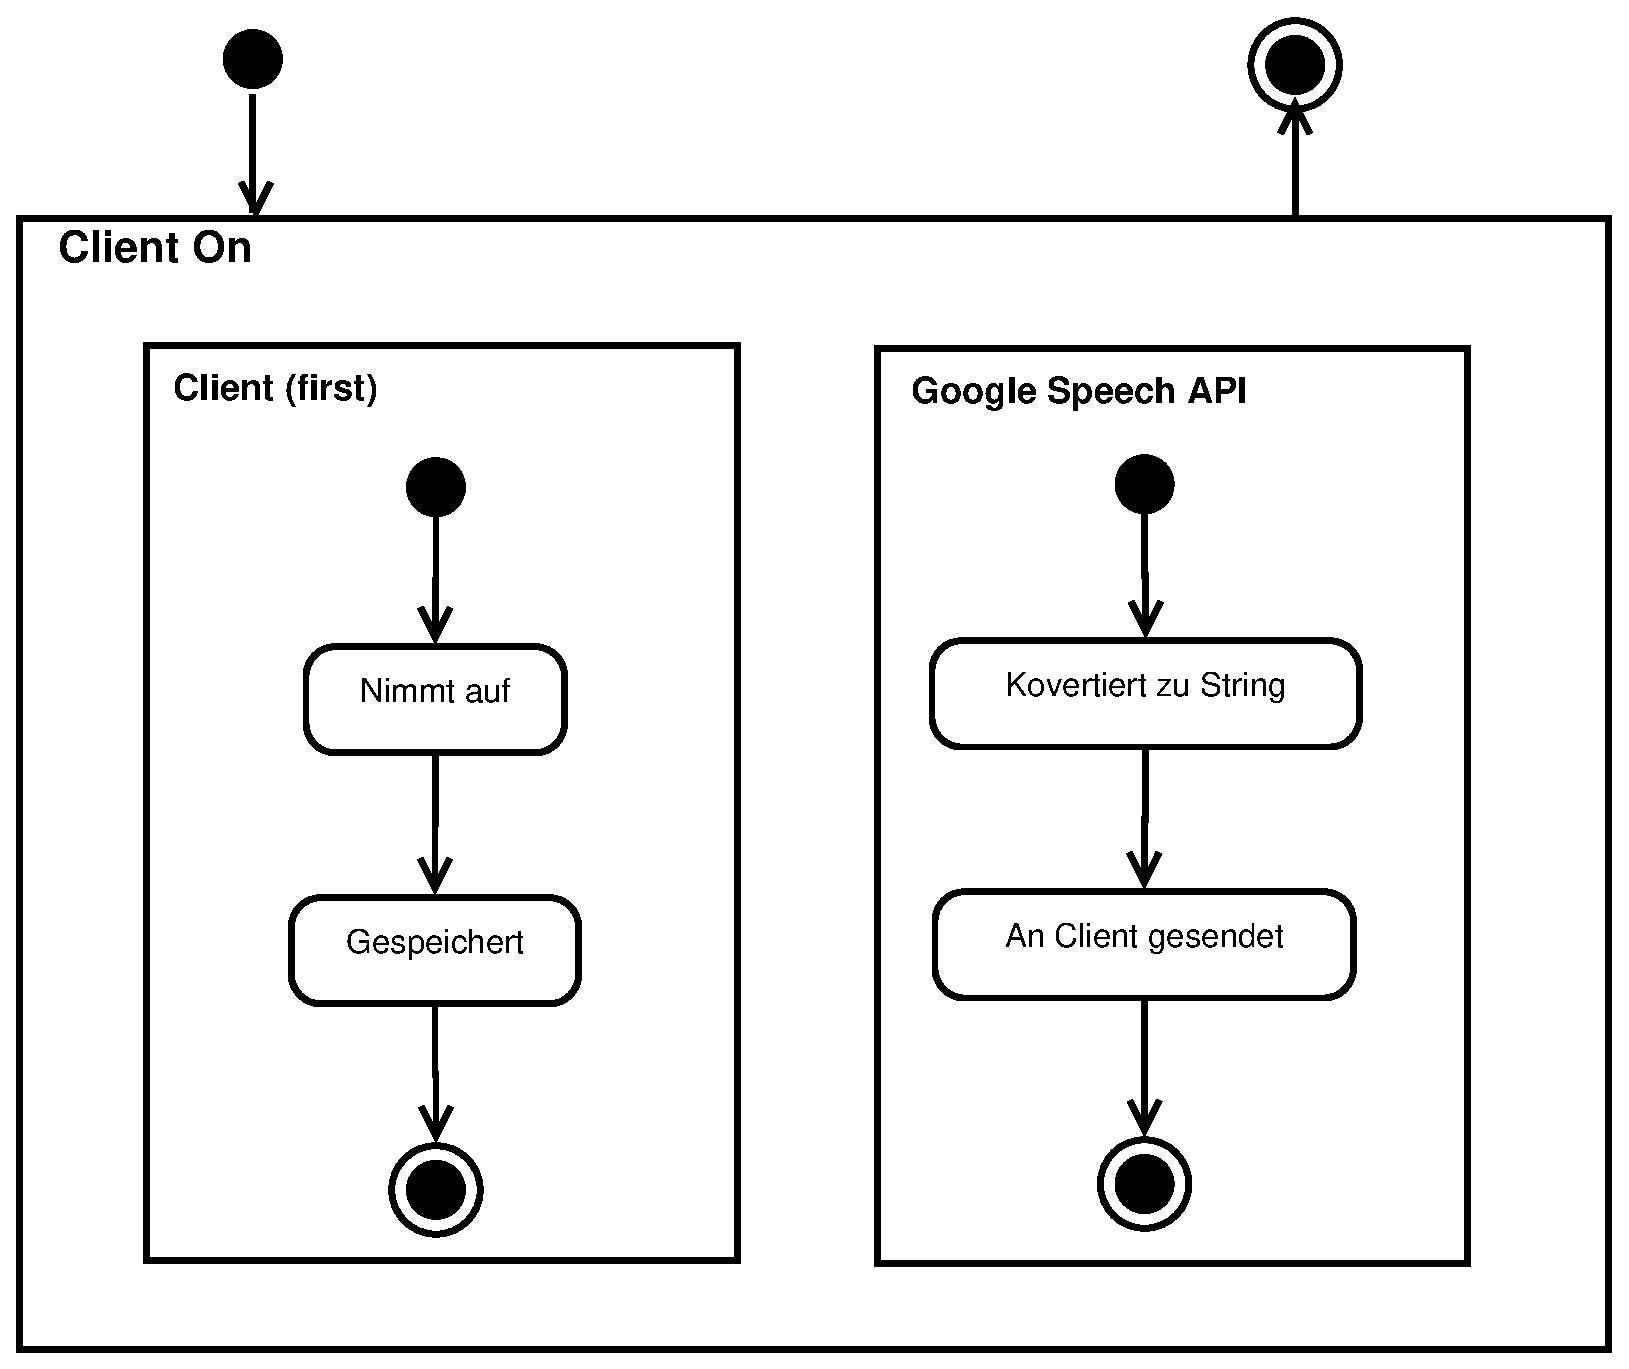
\includegraphics[width=.7\textwidth]{figures/client_chart.eps}
\caption{\textit{State Chart: Client}}
\label{fig:client_chart}
\end{figure}

\begin{figure}
\centering
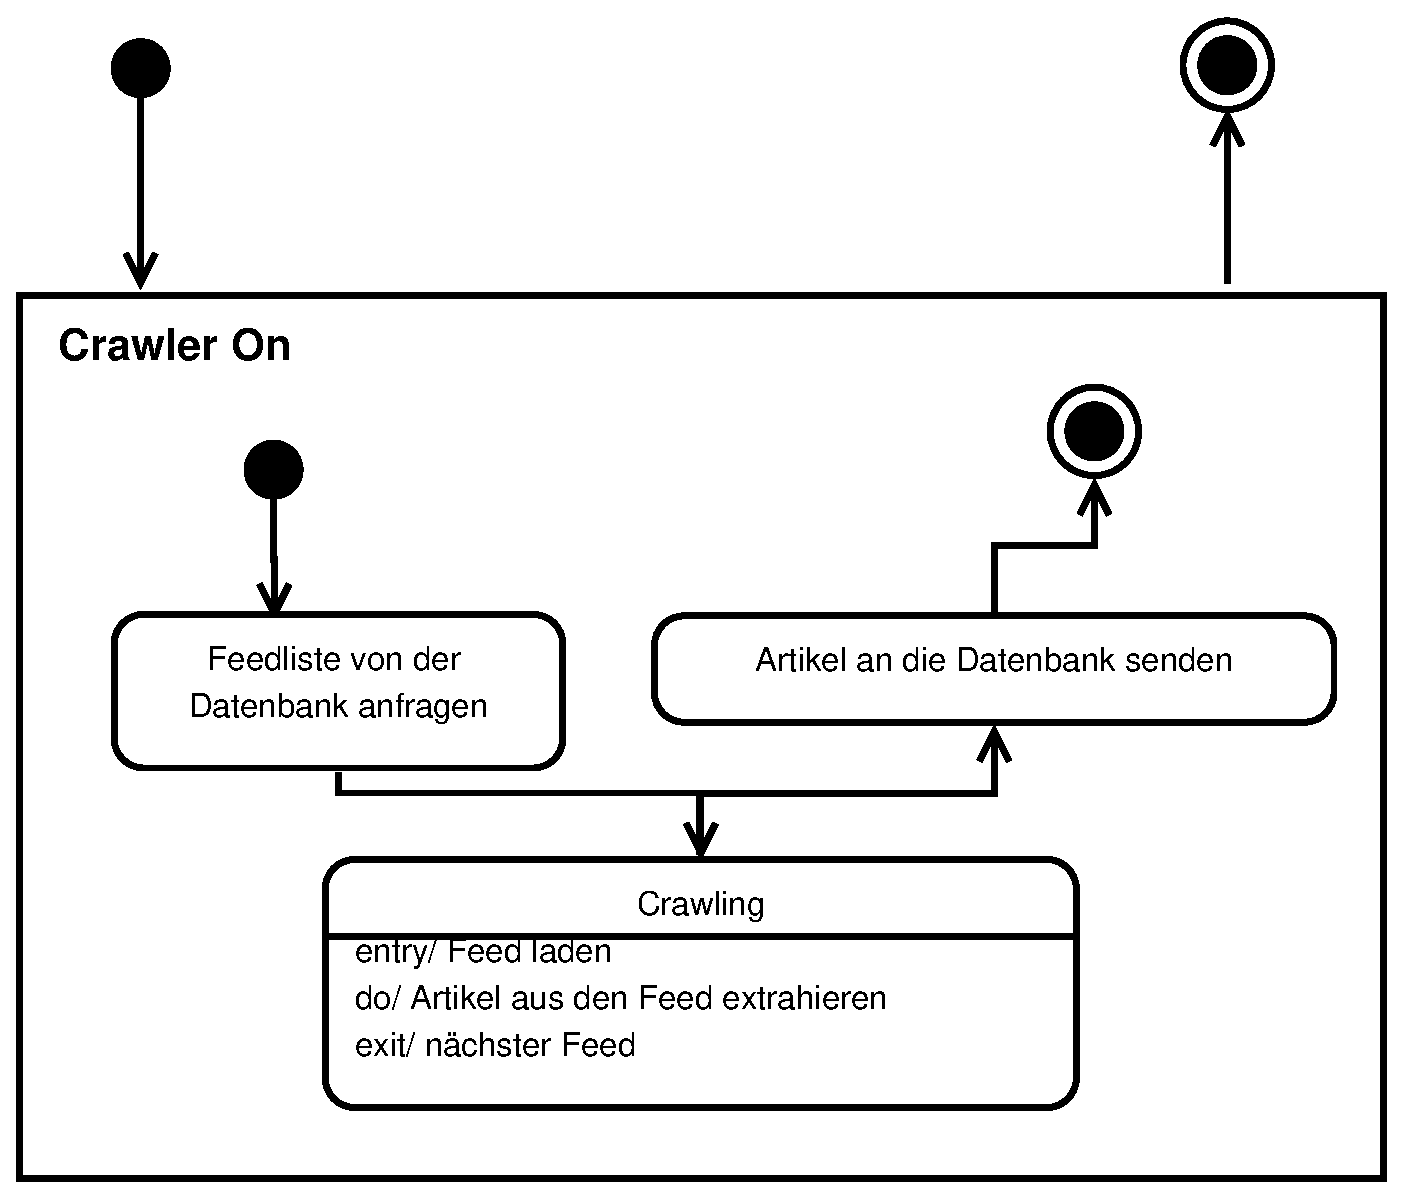
\includegraphics[width=0.7\textwidth]{figures/crawler_chart.eps}
\caption{\textit{State Chart: Crawler}}
\label{fig:crawler_chart}
\end{figure}



%!TEX root = ../TechnischerEntwurf.tex

\chapter{Verteilungsentwurf}

Das Front-End der Software sowie das mit gelieferte Admin-Tool wird über einen Webbrowser auf dem PC des Benutzers angezeigt. Die Daten dafür sind auf einem Server gespeichert. Um eingegebene Nutzerdaten zu überprüfen wird desweiteren eine Verbindung zum LDAP der TU Braunschweig aufgebaut.

\begin{figure}[ht]
\centering
\includegraphics[width=1\textwidth]{figures/Verteilung1.pdf}
\caption{Verteilungsdiagramm für SQL-Alchemst}
\label{deployment}
\end{figure}

%!TEX root = ../TechnischerEntwurf.tex

\chapter{Implementierungsentwurf}


\section{Implementierung von Komponente <C10>: Das Front-End:}

Im folgenden soll detailierter auf die Implementierung der Front-End-Komponente eingegenagen werden.

Das Front-End des SQL-Alchemisten beschreibt die Oberfläche der Applikation. Dabei wird darauf eingegangen, wie und an welcher Stelle das Front-End mit dem \hyperref[backend]{Back-End} kommuniziert. Außerdem wird detailliert das Layout der Software-Komponente beschrieben.

Bei der Entwicklung der Kompotente wird auf das MelonJS-Framework zurückgegriffen. Dieses ist ein Game-Framework.

Das gesamte Front-End ist aus folgenden Objekten aufgebaut:

\subsection{me.ScreenObject}
\label{ScreenObject}

In der Applikation befinden sich mehrere ScreenObjects. Diese stellen die einzelnen Bildschirme im Front-End dar. Jeder
Screen ist an einen STATE gekoppelt. Wird ein STATE gewechselt, so wird der entsprechende Screen geladen. Jeder Screen 
enth\"alt weitere Objekte die folgend erl\"autert werden. Dazu geh\"oren Container, HUDs, Buttons und Sprites. Au{\ss}erdem besitzt
jeder Screen ein eigenes Hintergrundbild welches direkt am Anfang des STATE-Changes geladen wird. Des Weiteren \"ubernehemen
alle Screen Objekte durch eine EXTENDS-Beziehung folgende Funktionen:
\begin{itemize}
	\item init() : Diese Funktion entspricht dem Konstruktor von Java-Klassen.
	\item onResetEvent() : Diese Funktion wird bei jedem Laden des Screens aufgerufen. Etwaige Ver\"anderungen in den Attributen 
	         werden hierbei ber\"ucksichtigt und aktualisiert.
	\item onDestroyEvent() : Das DestroyEvent beendet alle Prozesse die von den Attributen gestartet worden sind.           
	\item update() : Die Update-Funtktion f\"angt Ver\"anderungen w\"ahrend der Laufzeit des States ab und agiert dementsprechend.
	\item draw() : F\"ugt zus\"atzliche Elemente zu die Screens hinzu die nicht zu den Attributen geh\"oren. Das sind zum einen
		 zum Beispiel Bilder oder Texte.  
\end{itemize}

Folgende ScreenObjects existieren in der Applikation und sind vollst\"andig durch die Extends-Beziehung von me.ScreenObject
definiert. Diese sind in dem Digramm \ref {MEscreen} unter game.ScreenObjekt zusammengefasst.

\begin{itemize}
         \item game.StartScreen: Dieser Screen ist hat keine besonderen Funktionen und stellt in der Applikation nur einen 
                  Einf\"uhrungs-Screen dar. Man gelangt von diesem Screen mit dem STATE\_START-Zustand unmittelbar in den \nameref {Login}.
         \item game.ReadyScreen: Dieser Screen beschreibt das Labor im Story-Mode des Spiels und wird beim Wechseln in den READY-State
                  aufgerufen.
         \item game.PlayScreen: Der PlayScreen repr\"asentiert das Minispiel mit den Runs im Dungeon. Der dazugeh\"orige State ist der PLAY-
                  State. 
         \item game.BeltScreen: Dieser Screen soll den Tr\"anke-G\"urtel des Spielers repr\"asentieren. Hier werden dem Spieler all seine 
                  Potions angezeigt und es wird ihm die M\"oglichkeit gegeben diese in den Belt zu tun um sie im n\"achsten Run im Dungeon
                  zu verwenden. Erreicht wird dieser Screen durch den Wechsel in den "STATE\_BELT" Zustand.     
         \item game.CollectorScreen: In diesem Screen werden dem Spieler, sofern der Zustandswechsel in den STATE\_COLLECTOR-Zustand 
                  erfolgreich war, Informationen zu den eingesammelten Scrolls und Enchantmets, sowie dem f\"ur den Tag festgesetzten 
                  Scroll-Limit aufgezeigt.          
         \item game.GameOverScreen: Dieser Screen ist dazu da, um dem Spieler eine Zusammenfassung seines get\"atigten Runs zu geben.
                  Ihm werden die Anzahl der eingesammelten Scrolls und Enchantments, deren Namen, die Score und die Tiefe des Dungeons
                  angezeigt. Der dazugeh\"orige State ist in diesem Fall der GAMEOVER-State.
   	 \item game.TriviaScreen: W\"ahlt der Spieler diesen Screen (mit dem STATE\_TRIVIA-Zustand), so kann er SQL-Statements in 
        		  verschiedenen Schwierigkeitsstufen l\"osen. Hat der Spieler einen Schwierigkeitsgrad ausgew\"ahlt, so wird er durch einen 
       		  Zustandswechsel in den STATE\_TASK-Zustand in den \ref {task} Task-Screen umgeleitet.
   	 \item game.ResultScreen: Dieser Screen ist \"ahnlich wie der GameOverScreen. Hier bekommt der Spieler jedoch eine Zusammenfassung
        	          der Ergebnisse seines beantworteten SQL-Statements im \ref {task} TaskScreen. Dieser Zustand lautet dementsprechend STATE\_RESULT.
   	 \item game.HomeworkScreen: Dieser Screen (Zustand: STATE\_HOMEWORK) steht dem Spieler zur Hausaufgabenbearbeitung zur Verf\"ugung.
   	 \item game.SheetScreen: In diesem Screen (Zustand: STATE\_SHEET) hat der Spieler die M\"oglichkeit die Spielfigur zu \"andern.
   	 \item game.ShopScreen: Dieser Screen repr\"asentiert einen Shop in dem der Spieler zus\"atzliche Spielfiguren oder einen Beltslot 
                  dazukaufen kann. 
\end{itemize}

\newpage
\begin{figure}[ht]
\centering
\includegraphics[width=1.0\textwidth]{figures/KLassendiagrammScreens.pdf}
\caption{Klassendiagramm für die verschiedenen Screens}
\label{MEscreen}
\end{figure}

\newpage
Des Weiteren gibt es folgende Screens mit zus\"atzlichen Funktionen.

\subsection{game.AlertScreen}
\label{Alert}
Der AlertScreen (STATE\_ALERT) wird aufgerufen, sobald der User mit einem Fehler konfrontiert werden muss. Gibt der User zum Beispiel falsche Eingaben beim
Login oder SignUp an, so wird er mittels dieses Screens darauf hingewiesen. Dazu besitzt er die Funktion OnAlertOkClick(). Wird der Alert zur Kenntnis 
genommen, schickt diese Funktion den Spieler in den letzten ausgew\"ahlten State und der automatische Reset dieses Screens wird ausgef\"uhrt.

\subsection{game.HighscoreScreen}
\label{Score}
Als motivationsf\"ordernden Faktor bietet die Applikation die M\"oglichkeit Ranglisten einzusehen. Diese befinden sich im HisghscoreScreen 
(Zustand: HIGHSCORE). Dieser Screen besitzt folgende Funktionen, die die jeweilige Highscore-Ajax-Anfrage an den Server abf\"angt:
 \begin{itemize}
	\item scoreReply();
	\item coinsReply();
	\item timeSpentReply();
	\item runsReply();
	\item sqlStatementsReply();
	\item sqlRateReply();
\end{itemize}
HINWEIS: Es handelt sich hierbei immer um GET-Anfragen, das hei{\ss}t, bei diesen Anfragen kommen immer Informationen zur\"uck ohne das neben der 
Anfrage selbst vorher Informationen an den Server mitgesendet werden m\"ussen.
Au{\ss}erdem gibt besitzt der game.HighscoreScreen noch eine drawHighscore(xmlHttpRequest)-Funktion die als Parameter das zuvor abgefangene 
Ergebnis der Ajax-Anfrage bekommt und dieses via der draw()-Funktion visualisiert.

\newpage
\subsection{game.DefaultLoadingScreen}
\label{Loading}
Der DefaultLoadingScreen ist ein visuell an das SQL-Alchemist-Thema angepasster Lade-Bildschirm. Dieser Screen besitzt das Element Progressbar 
und enthlt die Funktion progress(). progress() ist eine Funktion, \"ahnlich der update()-Funktion, mit dem prozentualen Fortschritt des Ladevorganges 
als Updatevariable, welche in game.js load() gestartet wird.

\subsection{game.LoginScreen}
\label{Login}
Dieser Screen (STATE\_LOGIN) bietet die Funktionalit\"at des Einloggens in die Applikation. Au{\ss}erdem wird dem Spieler hier die M\"oglichkeit gegeben 
durch einen entsprechenden Zustands-Wechsel in den STATE\_SIGNUP in den \nameref {SignUp} zu gelangen.
Die zus\"atzlichen Funktionen sind:
\begin{itemize}
	\item loginReply(): Diese Funktion f\"uhrt den Login aus. Sie ist daf\"ur zust\"andig die f\"ur den Login notwendigen Daten aus den
	         daf\"ur vorhandenen TextInputElemente (einfache Texteingabefelder) zu filtern, diese in ein JSON-Objekt zu parsen und per 
      		Ajax-POST-Anfgrage an den Server zu senden.
	\item onLogin(xmlHttpRequest): Die Funktion onLogin(xmlHttpRequest) bekommt als Parameter die Antwort der Ajax-Anfrage. Wenn 
	         dieser erfolgreich war \"andert die Funktion den STATE\_MENU und der\nameref {Title} wird geladen.
	\item clearUserIdField() und clearPasswordField(): Diese Funktionen dienen rein optischen Zwecken. Sie sorgen daf\"ur, dass der
      		 sogenannte Placeholder in den TextInputElements verschwindet und der User ungest\"ort seine Login-Daten eingeben kann. 
\end{itemize}

\subsection{game.SignUpScreen}
\label{SignUp}
Dieser Screen (STATE\_SIGNUP) bietet Funktionalit\"at des Registrierens f\"ur die Applikation. Nach Erfolg gelangt man in den TItleScreen. 
Daf\"ur notwendige Funktionen sind:
\begin{itemize}  
	\item submitReply() und onSubmit() sind f\"ur den SignUp \"aqiuvalente Funktionen zum \nameref {Login} .
 	\item clearUserIdField(), clearUserNameField(), clearPasswordField() und clearPasswordAckField() sind ebenfalls \"aquivalente Funktionen
	         zum L\"oschen der Placeholder. 
\end{itemize}  

\subsection{game.SettingsScreen}
\label{Settings}  
Der SeetingsScreen bietet dem User die M\"oglichkeit seine Spieleinstellungen zu \"andern. Der User kann Sound- und Musikeinstellungen \"andern und
au{\ss}erdem auch noch sein Passwort sowoh\"o zu \"andern, als auch es zur\"uckzusetzen. Um diese Funktionalit\"at zu gew\"ahrleisten fibt es folgende
Funktionen:
\begin{itemize}    
	\item changePasswordClicked(): Diese Funktion \"offnet drei Textfelder: oldPassword, newPassword und newPasswordAck. Diese sind f\"ur eine 
		 erfolgreiche Passwort\"anderung n\"otig.
	\item submitPasswordClicked(): Diese Funktion kontrolliert das neue Passw\"ort und dessen Best\"atigung. Sollten die \"ubereinstimmen wird userReply() 
		 aufgerufen.
	\item userReply(xmlHttpRequest): Diese Funktion sendet das neue Passwort per Ajax-Anfrage zum Server.
\end{itemize}    

\subsection{game.ProfileScreen}
\label{Profile}  
Im ProfileScreen werden dem User s\"amtliche Profilinformationen angezeigt. Daf\"ur existiert die Funktion profileReply(), die alle entsprechenden Daten
von dem Server bekommt. Dazu f\"uhrt diese Funktion eine Ajax-.Anfrage aus. Bei Erfolg werden die Profilinformationen mittels draw()-Funktion visualisiert.

\newpage
\subsection{game.TaskScreen}
\label{Task}  
Der TaskScreen repr\"asentiert in der Applikation den SQL-Trainer. f\"ur die Funktionalit\"at existieren folgende Funktionen:
\begin{itemize} 
	\item getTaskFromServer(): Diese Funktion sendet die Ajax-Anfrage an den Server und f\"uhrt im Anschluss writeHeadline() aus. Das Ergebnis der Anfrage wird
		an handleGetTask() als xhr Parameter \"ubergeben.
	\item handleGetTask(xhr): Diese Funktion f\"angt das Ergebnis der Anfrage ab. Dieses enth\"alt die zu l\"osende SQL-Aufgabe.
	\item writeHeadline(): Die Funktion schreibt die \"Uberschrift basierend auf die Aufgabe in den Screen.      
	\item toggleSchemaButtonWithTaskButton(): Mit Hilfe dieser Funktion kann der User zwischen der Anzeige des Aufgabentextes und des relationellen Schema 
		wechseln.
	\item submitAnswer(): Diese Funktion sendet die L\"osung des Users an den Server. Dies geschieht auch hier wieder \"uber eine Ajax-Anfrage.
	\item clearInputField(): Diese Funktion l\"oscht wie im \nameref {Login} beziehungsweise dem \nameref {SignUp} bereits erw\"ahnt den Placeholder des Texteingabefeldes.
\end{itemize}        

\subsection{game.TitleScreen}
\label{Title}  
Der TitleScreen beschreibt die Men\"uf\"uhrung der Applikation. Alle Buttons die einen durch einen Zustandswechsel in andere STATES und somit in andere Screens l
eitet, sind durch verschiedene Bilder dargestellt. Wichtige Funktionen die hier verwendet werden sind:
\begin{itemize} 
	\item logoutReply(): Diese Funktion sendet die Ajax-POST-Anfrage zum Logout an den Server. Bei Erfolg wird die beim Login erstellte User Session gel\"oscht.
	\item onLogout(xmlHttpRequest): Diese Funktion f\"angt das Ergebnis der Anfrage ab und der User wird den LoginScreen geleitet.
\end{itemize}    

\newpage
\subsection{me.GUI\_Object}
\label{GUI}
In den oben beschriebenen ScreenObjects befinden sich verschiedene Buttons. Die verwendeten Buttons stehen, wie in Abbildung \ref {MEgui} zu sehen is, mit einer EXTENDS-Beziehung
zu me.GUI\_Object in Verbindung. Alle Buttons erben von me.GUI\_Object die Funktion onClick() die ausgef\"uhrt wird, wenn der Button
geklickt wird. Alle Atrribute die an alle Buttons vererbt werden sind:
\begin{itemize} 
	\item settings.image: Diese Attribut enth\"alt den String mit dem Name des Bildes welches in den Hintergrund des Buttons geladen wird.
	\item settings.spriteheight : Dieses Attribut definiert die H\"ohe des Buttons.
  	\item settings.spritewidth: Dieses Attribut definiert dementsprechend die Breite des Buttons.
 	\item z: Der z-Index beschreibt die H\"ohe des Layers im Canvas. Niedrigere z-Indizes werden hierbei immer von gr\"o{\ss}eren \"uberschrieben.
\end{itemize}       
  
Folgende Buttons existieren in der Applikation und sind vollst\"andig durch die Extends-Beziehung definiert:
\begin{itemize} 
	\item task: Dieser Button \"ubergibt die Taskvariable difficulty und startet den STATE\_TASK.
	\item skinLeft: Dieser Button befindet sich im SheetScreen und geht die Liste an vorhandenen Avataren nach links ab.
	\item skinRight: Dieser Button ist der entsprechenden Button der die Liste der Avatare nach rechts durchgeht.
	\item potionArrow: Dieser Button wird durch einen kleinen Pfeil dargestellt, besitzt das Attribut currentPotion und ist in der Lage den ausgew\"ahlten Potion in 
		den ersten freien BeltSlot zu verschieben.
	\item beltSlotBelt: Dieser Button befindet sich im BeltScreen, besitzt ebenfalls das Attribut des zugeh\"origen Beltslot und hat besitzt die gegenteilige Funktion zum 
		potion Arrow. Der Button verschiebt den Inhalt des Beltslots in die PotionCollection.
	\item showPotion: showPotion befindet sich im BeltScreen. Die onClick()-Funktion auf den entsprechenden Potion \"ubergibt die  Taskvariblen (potionId und 
		difficulty) an den TaskScreen und startet diesen.
	\item next: next befindet sich im ResultScreen definiert eine einfache Weiterleitung in den TaskScreen.
	\item backToMenu: Dieser Button befindet sich in verschiedenen Screen. M\"ochte der User aus s\"amtlichen Screens zur\"uck in das Men\"u gelangen, so ist
		diese Funktionalit\"at durch diesen Button gegeben.
	\item backToLab: Dieser Button befindet sich ebenfalls auf verschiedenen Screens. durch einen Klick auf diesen, gelangt der User zur\"uck in das Laboratory.
\end{itemize}     

Au{\ss}erdem existieren Buttons in der Applikation die zus\"atzliche update()-Funktion besitzen. Diese Funktion f\"angt ein Event ab und agiert dementsprechend.
Die Events sind so definiert, dass sie durch Tastendruck aktiviert werden k\"onnen.
 
Diese Buttons sind:
\begin{itemize} 
  	\item exit: Dieser Button befindet sich im PlayScreen. Die zugewiesene Event-Taste ist die ESC-Taste. Diese beendet den Zustand PLAY und startet STATE\_GAMEOVER.
  	\item music: music befindet sich im PlayScreen mit dem Buchstaben M als EventTaste. Sie deaktiviert beziehungsweise reaktiviert die Hintergrundmusik des Minispiels.
	\item sound: sound befindet sich ebenfalls im PlayScreen und besitzt den Buchstaben N als EventTaste. Sie deaktiviert beziehungsweise reaktiviert die Soundeffekte des Minispiels.
  	\item beltSlot: Dieser Button befindet sich im PlayScreen. Es besitzt das Attribut n mit 1,2,3,...,n der den beltSlot des Uses definiert. Die EventTasten
	werden von Q bis R dem entsprechenden Slots zugewiesen, sodass der User die eingebundenen Potions im Spiel benutzen kann.
\end{itemize} 

\newpage
\begin{figure}[ht]
\centering
\includegraphics[width=1.0\textwidth]{figures/KlassendiagrammButtons.pdf}
\caption{Klassendiagramm für die verschiedenen Screens}
\label{MEgui}
\end{figure}    

\newpage
\subsection{me.Entity}
\label{Entity}
In dem Minispiel befinden sich diverse Entit\"aten. Diese stehen alle in einer EXTENDS-Beziehung mit me.Entity in Verbindung.
me.Entity besitzt folgende Variablen die an alle Entit\"aten vererbt werden:
\begin{itemize} 
	\item name: Die Variable name vom Typ String beschreibt den Namen der Entit\"at.
	\item body.collisionType: Dieses Attribut legt fest wie sich die Entit\"aten verhalten wenn sie kollidieren.
	\item body.velocity: Dieses Attribut besteht aus zwei Werten x und  y vom Typ Integer. Diese beschreiben die Bewegung der Entit\"at in horizontaler (x) 
		beziehungsweise vertikaler (y) Ebene.
 	\item alive: Die Variable alive vom Typ Boolean beschreibt, ob die Entity existiert. Der Default-Wert der Variable ist hierbei immer true.
\end{itemize}    

Au{\ss}erdem wird die Funktion init(), die dem Konstruktor in Java-Klassen entspricht, an die Entit\"aten vererbt. Sie definiert die Koordinaten und auf welcher Map
die Entit\"aten erzeugt werden.
  
Die einzelnen Entit\"aten im Minispiel sind folgende:

\newpage
\subsection{game.PlayerEntity}
\label{PlayerEntity}
Die PlayerEntity beschreibt die Spielfigur mit der der User durch das Dungeon l\"auft. Sie besitzt folgende zus\"atzliche Variablen und Funktionen:
\begin{itemize} 
 	\item alwaysUpdate: Diese Variable vom Typ Boolean wird abgefragt, wenn sich der Spieler au{\ss}erhalb des Viewports (Bildschirm) befindet. 
		Ist dieser Wert true, wird die update()-Funktion der Entity ausgef\"uhrt.
 	\item hurt: Dieses Attribut vom Typ  Boolean wird genau dann auf true gesetzt wenn der Spieler mit einem Gegner kollidiert. Um ein erneutes Aufrufen 
		der onCollision()-Funktion zu verhindern, wird nach einiger Zeit das hurt-Attribut auf false gesetzt.
 	\item settings.image: Diese Variable vom Typ String definiert den Namen des Bildes der Spielfigur.
  
 	\item update(dt): Die Funktion bekommt den Parameter dt \"ubergeben. Dies ist eine Zeitvariable, die definiert in welchen Abs\"anden die update-Funktion
		 ausgef\"uhrt werden soll. Sie aktualisiert die Position der Figur abh\"angig von der body.velocity und f\"angt das Jump-Event ab (wenn die Spielfigur 
		 zum Springen gebracht wurde). Au{\ss}erdem \"uberpr\"uft die Funktion ob die Hitbox der Spielfigur sich mit der einer anderen Entit\"at schneidet.               
                 Sie gibt true zur\"uck,  wenn die Verschiebung gerendert werden konnte.
               
 	\item onCollision(): Die Funktion analysiert wie und mit welcher Entit\"at die PlayerEntity kollidiert ist und reagiert dementsprechend. Sie gibt true zur\"uck, 
		wenn die PlayerEntity mit einem festen Element wie den B\"oden, den W\"anden und der Decke, kollidiert. Das Ergebnis ist false, wenn es 
		stattdessen eine andere Entit\"at war.
\end{itemize}    

\newpage
\subsection{game.LevelEntity}
\label{LevelEntity}
Die game.LevelEntity beschreibt das Wechseln der Level am Ende jeder Map. Kollidiert die PlayerEntity mit der LevelEntity so \"andert sich die Map.
Die zus\"atzlichen Variablen und Funktionen, die die LevelEntity besitzt, sind:
\begin{itemize} 
	\item goToLevel: Die Variable vom Typ String beschreibt den Namen der nach der Kollision zu ladenden Map.
	\item settings.to: Diese Variabel vom Typ Integer \"ubergibt die Schwierigkeit des n\"achsten Levels.
	\item settings.fade: Dieses Attribut vom Typ String beschreibt die Farbe des Fades in RGB-Werten.
	\item settings.duration: beschreibt die L\"ange des Fades in Millisekunden.

  	\item findNextLevel(): Die Funktion sucht zuf\"allig eine Map f\"ur das n\"achste Level eines gewissen Schwierigkeitsgrades aus. Sie gibt den Namen 
		der n\"achsten Map als String. Dieser Name wird in goToLevel gespeichert.
\end{itemize}    

\subsection{game.CoinEntity}
\label{CoinEntity}                               
game.CoinEntity, ist eine "Collectable Entity". Sie erh\"oht den Score des Users und wird beim Kollidieren mit der PlayerEntity gel\"oscht.
Die zus\"atzliche Funktion die nicht direkt von me.Entity geerbt wird, ist die onCollision()-Funktion. Sie wird durch das Kollidieren mit der PlayerEntity
 ausgel\"ost und erh\"oht den Score des Users.

\newpage
\subsection{game.SpikeEntity}
\label{SpikeEntity}                            
Die game.SpikeEntity ist ebenfalls eine "Collectable Entity". Die beendet den Lauf im Dungeon beim Kollidieren mit der PlayerEntity.
Auch diese Entit\"at besitzt die zus\"atzliche onCollision()-Funktion. Diese beendet den Lauf des Spielers und f\"uhrt einen Zustandswechsel in
den GAMEOVER-State

\subsection{game.ScrollEntity}
\label{ScrollEntity}    
Auch die game.ScrollEntity, ist eine "Collectable Entity". Der User sammelt diese ein und sie wird beim Kollidieren mit der PlayerEntity aus der Map entfernt.
Die zus\"atlichen Variablen und Funktionen sind:
\begin{itemize} 
	\item settings.scrollIndex: Diese Variable enth\"alt eine eindeutige ID der Scroll.
	\item settings.type: Diese Variable vom Typ String beschreibt den Typ der Scroll. Sie ist entweder eine  "Potion"-Scroll oder eine "Entchantent"-Scroll
	\item onCollision(): Diese Funktion wird durch das Kollidieren mit der PlayerEntity ausgel\"ost. Sie speichert die Scroll f\"ur den User und entfernt die Entity. 
\end{itemize}                      

\subsection{game.EnemyEntity}
\label{EnemyEntity}    
Die game.EnemyEntity beschreibt alle Gegner-Entit\"aten die im Minispiel vorkommen.
Die zus\"atzlichen Attribute und Funktionen die diese Entit\"aten besitzen sind:
\begin{itemize} 
	\item settings.spritewidth: Dieses Attribut vom Typ Integer beschreibt die Breite des Sprites der die Entit\"at im Spiel darstellt.
	\item settings.spriteheight: Dieses Attribut beschreibt entsprechend zur Breite des Sprites Die  H\"ohe.
	\item settings.jump: Das Attribut ist vom Typ Integer und definiert die Geschwindigkeit in vertikaler Ebene.
	\item settings.speed: Dieses Attribut beschreibt die Geschwindigkeit der Entit\"at in horizontaler Ebene.
	\item settings.attack: Integer: Diese Eigenschaft definiert die H\"ohe des Schadens den der Spieler bekommt, wenn er mit der EnemyEntity kollidiert.
	\item startY: Dieses Attribut vom Typ Integer entspricht der y-Koordinate von me.Entity bei der Initiallisierung.
	\item startX: Dieses Attribut vom Typ Integer entspricht dementsprechend der x-Koordinate von me.Entity.
	\item pos.Y: In dieser Variable wird die aktuelle y-Koordinate der Entit\"at gespeichert.
	\item pos.X: In dieser Variable wird dementsprechend die x-Koordinate der Entit\"at gespeichert.
	\item endY: endY vom Typ Integer beschreibt die y-Koordinate, welche das Ende des Bereiches, in welchem sich die Gegner-Entit\"at bewegen darf.
	\item endX: endX ist entsprechend zu endY die x-Koordinate des Bereichs in der sich die Entit\"at bewegen darf.
	\item jump: Dieses Attribut vom Typ Boolean wird genau dann auf true gesetzt, wenn die Gegner-Entit\"at spring beziehungsweise fliegt und false wenn 
		sie f\"allt. Der Default-Wert dieser Variable ist false gesetzt.
	\item walkLeft: Dieses Attribut vom Typ Boolean wird auf Ist true gesetzt, wenn sich die Gegner-Entit\"at nach links bewegt und false wenn sie 
		nach rechts geht. Auch dieses Attribut ist stndartm\"a{\ss}ig auf false gesetzt. 
	\item update(): Diese Funktion l\"ast die EnemyEntity nach links laufen und fliegen. Erreicht die Entit\"at endY oder endX kehrt sie um l\"auft nach 
		rechts und f\"allt bis zu startY und startX. Die Funktion gibt true zur\"uck wenn das Rendern der Entit\"at auf der neuen Position erfolgreich war.
	\item body.setVelocity(): Diese Funktion legt horizontale und vertikale Bewegungen fest.
\end{itemize}  


\newpage
\begin{figure}[ht]
\centering
\includegraphics[width=1.0\textwidth]{figures/KlassendiagrammFrontEndEntities.pdf}
\caption{Klassendiagramm für die verschiedenen Front-End-Entitäten}
\label{MEentity}
\end{figure}   

\newpage    

% HERE BEGIN


%\subsection{game.me.Container}
%Container sind da um verschiedene HUDs und buttons zu b¸ndeln und ihnen gemeinsame Eigenschaften zu geben. Die Eigenschaften der HUDs
%und buttons werden an deren Stellen genauer beschrieben.
%Sie besitzen folgende Variablen:
 % - isPersistent: Boolean: Wenn true kann der Contaier nicht ver‰ndert werden.
 % - floating: Boolean: Wenn true bewegen sich die Elemente des Containers mit dem Viewport(Spierler Bildschirm) mit.
 % - name: String: Name des Containers.
%  - z: Integer: Beschreibt die Hˆhe in welcher Element des Containers in den Canvas geladen werden.
%und die Konstruktorfunktion:
 % - init(): Entspricht dem Konstruktor in Java.
  
%In der Applikation befinden sich 2 Container alle extenden von me.Container deren.
%Die Container werden im Minispiel eingeladen.
 
%- game.HUD.Container
%In den Container werden folgende HUDs eingetragen
 % - HUD.ScoreItem
  %- HUD.HealthScore

% - game.HUDII.Container
%In den Container werden folgende Buttons eingetragen
% - beltSlots
% - sound
% - music
% - exit
 
%me.Sprite
%Bilder die ohne jegliche besondere Eigenschaften eingeladen werden.
%Sie besitzen folgende Variablen:
%  - z: Integer: Beschreibt die Hˆhe in welcher Element des Containers in den Canvas geladen werden.
%und die Konstruktorfunktion:
%  - init(): Entspricht dem Konstruktor in Java.
  
%game.Icon extendet von me.Sprite

%game.SkinFront
%besitzt folgende Variablen:
%  - currentSkin: String: Name des Skins. Wird als Updatevariable benutzt.
%und folgende Funktion:
%  - update(dt): Der Parameter: dt ist die Zeitvariable in welchen Abst‰nden update ausgef¸hrt wird.
%                L‰dt das Bild neu wenn es ge‰ndert wird.


%END HERE      
          
\subsection{me.Renderable}
\label{Render}                   
Alle HUDs (Head-Up-Displays) stehen in einer EXTENDS-Beziehung zu me.Renderable. HUDs werden in derApplikation daf\"ur verwendet, Texte zu 
in die Screens zu schreiben und diese zur Laufzeit zu aktualisieren.
Sie besitzen folgende Variablen und Funktionen:
\begin{itemize} 
	\item font: Das font-Attribut enth\"alt dem Schrifttyp der in der draw()-Funktion benutzt wird.
	\item init(): Diese Funktion entspricht dem Konstruktor in Java und initialisiert das HUD.
	\item update(): Diese Funktion aktualisiert das HUD. Sie gibt true zur\"uck, wenn der eingef\"ugte Text erfolgreich gerendert werden konnte.
	\item draw(): Diese Funktion enth\"alt den Text der auf das HUD geschrieben werden soll.
\end{itemize}                     

Alle HUDs die von me.Renderable erben sind:
\begin{itemize} 
	\item game.HUD.ScoreItem: Dieses HUD schreibt den Score des Spielers das im Minispiel angezeigt wird.
	\item game.HUD.HealthScore: Dieses HUD schreibt die Leben die der User aktuell im Minispiel besitzt.
	\item game.HUD.SkinName: Dieses HUD schreibt den Namen des entsprechenden, ausgew\"ahlten Avatares. Es wird im SheetScreen verwendet.
	\item game.HUD.SettingsElements: Dieses HUD schreibt die Einstellungen des User in den \nameref {Settings}.
	\item game.HUD.GameOver: Dieses HUD schreibt alle Informationen des GameOverScreens.
	\item game.HUD.Result: Dieses HUD schreibt den Inhalt des ResultScreens.
	\item game.HUD.Profile: Der Inhalt des \nameref {Profile} werden in diesem HUD geschrieben.
	\item game.HUD.PotionAmount: Dieses HUD schreibt die Anzahl der vorhanden Potions in den BeltScreen.
	\item game.HUD.Shop: Dieses HUD schreibt die Anzahl der Lofi-Coins in den ShopScreen.
	\item game.HUD.OverlayAlert: Dieses HUD schreibt die Fehlermeldungen in den AlertScreen.
\end{itemize} 

\newpage
\begin{figure}[ht]
\centering
\includegraphics[width=1.0\textwidth]{figures/KLassendiagrammRenderables.pdf}
\caption{Klassendiagramm für die Renderables}
\label{MErenderable}
\end{figure}    

\newpage


\newpage
\section{Implementierung von Komponente <C20>: Das Back-End}
\label{backend}

Im folgenden Abschnitt soll detaillierter auf die Implementierung der Back-End-Komponente eingegangen werden.

Das Back-End des SQL-Alchemist hat die Aufgabe, die spielinterne Datenbank zu verwalten. Dabei müssen die anfallenden Daten korrekt gespeichert und dem Front-End auf Anfrage zur Verfügung gestellt werden.

Bei der Entwicklung dieser Komponente wird auf zwei Bibliotheken zurückgegriffen. Zunächst gehört dazu das play!-Framework, welches dazu dient webbasierte Anwendungen zu erstellen. Dabei stellt es zusätzlich auch die im Projekt verwendete Datenbank zur Verfügung. Die zweite verwendete Bibliothek wird vom Teamprojekt entwickelt und prüft SQL-Statements auf ihre Korrektheit. Dies wird beim SQL-Modul des SQL-Alchemisten Anwendung finden. 

Im ersten Unterkapitel wird die Komponente durch Klassendiagramme dargestellt. Der Übersicht halber wurden die Klassen dabei auf mehrere Diagramme verteilt, da der Umfang der Komponente den Rahmen einer Seite übersteigen würde. Um den Zusammenhang der einzelnen Diagramme untereinander zu verdeutlichen werden Klassen, die Assoziationen zu Klassen in anderen Diagrammen haben, in diesen ebenfalls, aber ohne Attribute und Methoden, dargestellt.  

Im zweiten Unterkapitel werden dann jeweils noch kurz die einzelnen Klassen, sowie deren Attribute und Methoden beschrieben.

\clearpage


\newpage


\subsection{Model Classes -- Profile}
\subsection{Paket-/Klassendiagramm}
\begin{figure}[h!]
\centering
\includegraphics[width=0.8\textwidth]{figures/KDProfile}
\caption{Klassendiagramm für die Model-Klasse Profile \ref{C20}}
\label{classC10}
\end{figure}
\clearpage
\subsection{Erläuterung}
\begin{class}{10}{Profile}
\item[Aufgabe]~\\
Verwaltung der Nutzerprofile des SQL-Alchemist
\item[Attribute]~\\
\begin{itemize}
\item id:long -- Einzigartige ID
\item username: String -- Benutzername des zugehörigen Nutzers
\item coinsCollected: int -- Anzahl der bisher gesammelten Lofi-Coins
\item coins: int -- Anzahl der momentanen Lofi-Coins des Nutzers
\item coinScale: float -- 
\item scrollLimit: int -- Anzahl der maximal sammelbaren Schriftrollen pro Zeitraum
\item points: int -- Die Punkte des Spielers
\item playerStats: PlayerStats -- Die Attribute der Spielfigur des Nutzers
\item settings: Settings -- Die vom Nutzer gewählten Einstellungen
\item avatar: Avatar -- Der vom Nutzer gewählte Avatar
\item shopItems: List<ShopItem> -- Bisher vom Nutzer gekaufte Gegenstände
\item tutorialDone: boolean -- Hält fest ob das Tutorial bereits vom Nutzer bearbeitet wurde
\item user: User -- Der zum Profil gehörige Nutzer
\item created\_at: Date -- Zeitpunkt zu dem das Profil erstellt wurde
\item edited\_at: Date -- Zeitpunkt zu dem das Profil zuletzt bearbeitet wurde
\item totalPoints: int -- Gesamtzahl der vom Nutzer erspielten Punkte
\item playedTime: int -- Bisher im Spiel verbrachte Zeit
\item playedRuns: int -- Bisher gespielte Durchläufe
\item doneSQL: int -- Bisher bearbeitete SQL-Aufgaben
\item solvedSQL: int -- Bisher korrekt gelöste SQL-Aufgaben
\item quote: float -- Rate von gelösten SQL-Aufgaben im Vergleich zu bearbeiteten Aufgaben
\item find: Finder<Long, Profile> -- Der Finder der Klasse zum Suchen in der Datenbank
\end{itemize}
\item[Operationen]~\\
\begin{itemize}
\item save() -- Diese Methode speichert das Profil
\item toJsonProfile(): ObjectNode -- Erzeugt aus einem Profildatensatz ein Json-Objekt
\item toJsonPlayerState(): ObjectNode -- Erzeugt aus einem Profildatensatz ein auf den PlayerState spezialisiertes Json-Objekt
\item toJsonBoughtAvatars(): ArrayNode -- Erzeugt ein Json-Array in welchem die gekauften Avatare gespeichert sind
\item toJsonCharacterState(): ObjectNode --
Erzeugt aus einem Profildatensatz ein auf den CharacterState spezialisiertes Json-Objekt
\item toJsonHighScore(): ObjectNode -- Erzeugt aus einem Profildatensatz ein für die Ranglisten spezialisiertes Json-Objekt
\item toJsonHighScoreAll(profiles: List<Profile>): ArrayNode -- Erstellt ein für die Ranglisten spezialisiertes Json-Array, welches mehrere Profileinträge enthält
\item getPlayerStats(): PlayerStats -- Kombiniert die PlayerStats des Avatars mit denen des Nutzers und gibt diese zurück
\item create(username: String, user: User): Profile -- Erstellt einen neuen Profildatensatz
\item getById(id: long): Profile -- Sucht ein Profil anhand dessen ID und gibt es zurück
\item shopItemInList(shopItem): boolean -- Prüft, ob ein ShopItem bereits gekauft wurde
\item sortByPoints(): List<Profile> -- Gibt eine Liste der, nach Punkten sortiert, zehn besten Profile zurück
\item sortByTime(): List<Profile> -- Gibt eine Liste der, nach Spielzeit sortiert, zehn besten Profile zurück
\item sortByRuns(): List<Profile> -- Gibt eine Liste der, nach Durchläufen sortiert, zehn besten Profile zurück
\item sortBySQL(): List<Profile> -- Gibt eine Liste der, nach gelösten SQL-Aufgaben sortiert, zehn besten Profile zurück
\item sortByRate(): List<Profile> -- Gibt eine Liste der, nach Erfolgsquote sortiert, zehn besten Profile zurück
\item sortByCoins(): List<Profile> -- Gibt eine Liste der, nach gesammelten Lofi-Coins sortiert, zehn besten Profile zurück
\item ListToArray(listToChange: List<Profile>): Profile[] -- Erzeugt ein Array aus einer Liste
\item ownRank(ownProfile: Profile): JsonNode -- Erzeugt ein für die Ranglisten spezialisiertes Json-Objekt
\item buy(shopItem: ShopItem): boolean -- Prüft, ob der Nutzer genügend Coins hat um ein ShopItem zu kaufen und führt dann den Kauf durch
\end{itemize}
\item[Kommunikationspartner]~\\
\begin{itemize}
\item EventChallenge
\item ShopItem
\item Avatar
\item User
\item Settings
\item PlayerStats
\item Challenge
\item SolvedTask
\item Task
\item Comment
\item Inventory
\end{itemize}
\end{class}

\newpage
\subsection{Model Classes -- Part 1}
\subsection{Paket-/Klassendiagramm}
\begin{figure}[h!]
\centering
\includegraphics[width=0.8\textwidth]{figures/KDChallenge}
\caption{Klassendiagramm für einige der Model-Klassen \ref{C20}}
\label{classC10}
\end{figure}
\clearpage
\subsection{Erläuterung}
\begin{class}{20}{Challenge}
\item[Aufgabe]~\\
Verwaltung der Aufgabenpakete
\item[Attribute]~\\
\begin{itemize}
\item id: long -- Einzigartige ID
\item solve\_type: int -- Beschreibt die Eigenschaften des Paketes hinsichtlich dessen Lösung
\item solve\_type\_extension: int -- Zusatz zu den Eigenschaften des Aufgabenpaketes
\item tasks: List<Task> -- Eine Liste der im Paket enthaltenen Aufgaben
\item created\_at: Date -- Zeitpunkt zu dem das Aufgabenpaket erstellt wurde
\item modified\_at: Date -- Zeitpunkt zu dem das Aufgabenpaket zuletzt geändert wurde
\item player: Profile -- Spieler, denen das Aufgabenpaket gestellt wird
\item find: Finder<Long, Challenge> -- Der Finder der Klasse zum Suchen in der Datenbank
\end{itemize}
\item[Operationen]~\\
\begin{itemize}
\item update() -- Aktualisiert das Aufgabenpaket
\item create(solve\_type: int, solve\_type\_extension: int) -- Erstellt ein neues Aufgabenpaket
\item getStory(profile: Profile): Challenge -- Gibt die Story zurück
\end{itemize}
\item[Kommunikationspartner]~\\
\begin{itemize}
\item Task
\item Profile
\item RandomChallenge
\item EventChallenge
\end{itemize}
\end{class}

\newpage
\begin{class}{30}{RandomChallenge}
\item[Aufgabe]~\\
Verwaltet das zufällige Stellen von Aufgabenpaketen
\item[Attribute]~\\
Keine
\item[Operationen]~\\
Keine
\item[Kommunikationspartner]~\\
\begin{itemize}
\item Challenge
\end{itemize}
\end{class}

\newpage
\begin{class}{40}{EventChallenge}
\item[Aufgabe]~\\
Verwaltung der Aufgabenpakete für spezielle Events
\item[Attribute]~\\
\begin{itemize}
\item name: String -- Name des Aufgabenpaketes
\item creator: Profile -- Der Nutzer, der das Paket erstellt hat
\item type: int -- Der Typ des Paketes
\item expires\_at: Date der Zeitpunkt, wann das Aufgabenpaket nicht mehr gelöst werden kann
\item find: Finder<Long, EventChallenge> -- Der Finder der Klasse zum Suchen in der Datenbank
\end{itemize}
\item[Operationen]~\\
\begin{itemize}
\item create(name: String, creator: Profile, solve\_type: int, solve\_type\_extension: int, tasks: List<Task>, type: int, expires\_at: Date): EventChallenge -- Erstellt ein neues Aufgabenpaket
\end{itemize}
\item[Kommunikationspartner]~\\
\begin{itemize}
\item Profile
\item Challenge
\item StoryChallenge
\end{itemize}
\end{class}

\newpage
\begin{class}{50}{StoryChallenge}
\item[Aufgabe]~\\
Verwaltung der Aufgabenpakete für den Story-Modus
\item[Attribute]~\\
\begin{itemize}
\item texts: List<Text> -- Eine Liste der im Aufgabenpaket verwendeten Texte
\item maps: List<Map> -- Eine Liste der im Aufgabenpaket verwendeten Karten
\item next: StoryChallenge -- Das Aufgabenpaket, welches auf das aktuelle folgt
\item find: Finder<Long, StoryChallenge> -- Der Finder der Klasse zum Suchen in der Datenbank
\end{itemize}
\item[Operationen]~\\
\begin{itemize}
\item toJson(): ObjectNode -- Erstellt aus dem Paket ein Json-Objekt
\item setTexts(texts: List<SimpleText>): boolean -- Fügt dem Paket neue Texte hinzu
\item create(name: String, tasks: List<Task>, isTutorial: boolean, texts: List<SimpleText>, maps: List<map>, next: StoryChallenge, expires\_at: Date): StoryChallenge -- Erstellt ein neues Aufgabenpaket
\item getForProfile(profile: Profile): StoryChallenge -- Weist das Aufgabenpaket einem Profil zu
\end{itemize}
\item[Kommunikationspartner]~\\
\begin{itemize}
\item Map
\item Text
\item EventChallenge
\end{itemize}
\end{class}

\newpage
\begin{class}{60}{Map}
\item[Aufgabe]~\\
Verwaltung der Minispiel-Karten
\item[Attribute]~\\
\begin{itemize}
\item id: long -- Einzigartige ID
\item level: int -- Gibt den Level dar, in dem die Karte verwendet wird
\item path: String -- Der Pfad an dem die Karte abgespeichert ist
\item isBossMap: boolean -- Legt fest, ob die Karte eine Karte mit Endgegner ist
\item find: Finder<Long, Map> -- Der Finder der Klasse zum Suchen in der Datenbank
\end{itemize}
\item[Operationen]~\\
\begin{itemize}
\item toJson(): ObjectNode -- Erstellt aus dem Kartendatensatz ein Json-Objekt
\item create(level: int, path: String): Map -- Erstellt einen neuen Kartendatensatz
\item create(level: int, path: String, isBossMap: boolean): Map -- Erstellt einen neuen Kartendatensatz
\item getById(id: long): Map -- Sucht eine Karte anhand ihrer ID
\item getByLevel(level: int): List<Map> -- Sucht alle Karten, die in einem bestimmten Level vorkommen
\item init() -- Initialisiert die Karten
\end{itemize}
\item[Kommunikationspartner]~\\
\begin{itemize}
\item StoryChallenge
\end{itemize}
\end{class}

\newpage
\begin{class}{70}{Text}
\item[Aufgabe]~\\
Verwaltung der Texte für den Story-Modus
\item[Attribute]~\\
\begin{itemize}
\item id: long -- Einzigartige ID
\item type: int -- Art des Textes
\item prerequisite: int -- Bedingung, die erfüllt sein muss, damit der Text aufgerufen wird
\item chronology: int -- Reihenfolge, in der die Texte auftreten
\item text: String -- Der eigentliche Text
\item sound\_url: String -- Der zum Text gehörende Sound
\item find: Finder<Long, Text> -- Der Finder der Klasse zum Suchen in der Datenbank
\end{itemize}
\item[Operationen]~\\
\begin{itemize}
\item toJson(): ObjectNode -- Erzeugt aus dem Textdatensatz ein Json-Objekt
\item create(type: int, chronology: int, prerequisite: int, text: String, sound\_url: String): Text -- Erstellt einen neuen Textdatensatz
\item getTextByType(type: int): Text -- Sucht einen zufälligen Text eines bestimmten Typs heraus und gibt ihn zurück
\item getTerrySuccessfull(): Text -- Sucht einen Text mit positiven Kommentar von Terry zurück
\item getTerryFailure(): Text -- Sucht einen Text mit negativen Kommentar von Terry zurück
\item getTerryUrge(): Text -- Sucht einen Text mit drängendem Kommentar von Terry zurück
\end{itemize}
\item[Kommunikationspartner]~\\
\begin{itemize}
\item StoryChallenge
\end{itemize}
\end{class}

\newpage
\subsection{Model Classes -- Part 2}
\subsection{Paket-/Klassendiagramm}
\begin{figure}[h!]
\centering
\includegraphics[width=0.8\textwidth]{figures/KDUserAndAvatar}
\caption{Klassendiagramm für einige der Model-Klassen \ref{C20}}
\label{classC10}
\end{figure}
\clearpage
\subsection{Erläuterung}
\begin{class}{80}{User}
\item[Aufgabe]~\\
Verwaltung der Nutzer
\item[Attribute]~\\
\begin{itemize}
\item id: long -- Einzigartige ID
\item email: String -- Email-Adresse des Nutzers
\item emailVerified: boolean -- Legt fest, ob die Adresse bereits verifiziert ist
\item emailVerifyCode: String -- Der Verifizierungscode der Adresse
\item y\_id: String -- Die y-Nummer des Nutzers (falls der Nutzer ein Student ist)
\item matNR: String -- Die Matrikelnummer des Nutzers (falls der Nutzer ein Student ist)
\item passwordHash: String -- Der Passwort-Hash des Nutzers
\item passwordResetCode: String -- Der Code zum Zurücksetzen des Passworts
\item role: int -- Rechtegruppe, welcher der Nutzer angehört
\item sessions: List<UserSession> -- Liste an Sitzungen, die der Nutzer gestartet hat
\item profile: Profile -- Das Profil des Nutzers
\item created\_at: Date -- Zeitpunkt zu dem sich der Nutzer registriert hat
\item edited\_at: Date -- Zeitpunkt zu dem zuletzt etwas am Nutzerdatensatz geändert wurde
\item find: Finder<Long, User> -- Der Finder der Klasse zum Suchen in der Datenbank
\end{itemize}
\item[Operationen]~\\
\begin{itemize}
\item changePassword(oldPassword: String, newPassword: String): boolean -- Methode zum Ändern des Passworts
\item setProfile(profile: Profile) -- Weist dem Nutzer ein Profil zu
\item isStudent(): boolean -- Prüft, ob der Nutzer ein Student ist
\item update() -- Aktualisiert den Nutzerdatensatz
\item create(username: String, id: String, password: String): User -- Erstellt einen neuen Nutzerdatensatz
\item create(username: String, id: String, password: String, role: int): User -- Erstellt einen neuen Nutzerdatensatz
\item getByEmail(email: String): User -- Sucht einen Nutzer anhand seiner Email-Adresse
\item getProfile(session: Http.Session): Profile -- Gibt das zu einer Sitzung gehörende Profil zurück
\item getByY\_ID(y\_ID: String): User -- Sucht einen Nutzer anhand seiner y-Nummer
\item validate(id: String, password: String): User -- Validiert einen Nutzer
\item resetPassword(email: String): boolean -- Setzt das Passwort des Nutzers zurück
\item verifyEmail(emailVerifyCode: String): int -- Verifiziert eine Email-Adresse
\end{itemize}
\item[Kommunikationspartner]~\\
\begin{itemize}
\item UserSession
\item Profile
\end{itemize}
\end{class}

\newpage
\begin{class}{90}{UserSession}
\item[Aufgabe]~\\
Verwaltung der durch die Nutzer gestarteten Sitzungen
\item[Attribute]~\\
\begin{itemize}
\item id: Long -- Einzigartige ID
\item sessionID: String -- Einzigartige Sitzungs-ID
\item user: User -- Nutzer der sie Sitzung gestartet hat
\item remoteAddress: String -- Netzwerkkennung des Nutzers
\item created\_at: Date -- Zeitpunkt zu dem die Sitzung gestartet wurde
\item expires\_at: Date -- Zeitpunkt zu dem die Sitzung geschlossen wird
\item find: Finder<Long, UserSession> -- Der Finder der Klasse zum Suchen in der Datenbank
\end{itemize}
\item[Operationen]~\\
\begin{itemize}
\item create(user: User, duration: Integer, remoteAddress: String): UserSession -- Erstellt eine neue Sitzung
\item isValid(remoteAddress: String): boolean -- Prüft ob die Sitzung gültig ist
\item getSession(session: Http.Session): UserSession -- Gibt die Sitzung zurück
\end{itemize}
\item[Kommunikationspartner]~\\
\begin{itemize}
\item User
\end{itemize}
\end{class}

\newpage
\begin{class}{100}{Avatar}
\item[Aufgabe]~\\
Verwaltung der Avatare
\item[Attribute]~\\
\begin{itemize}
\item id: long -- Einzigartige ID
\item name: String -- Name des Avatars
\item desc: String -- Beschreibung des Avatars
\item avatarURL: String -- Pfad, an dem der Avatar gespeichert wird
\item spriteURL: String -- Pfad, an dem der Sprite des Avatars abgespeichert wird
\item soundURL: String -- Pfad, an dem der Sound des Avatars abgespeichert wird
\item playerStats: PlayerStats -- Die Attribute des Avatars
\item find: Finder<Long, Avatar> -- Der Finder der Klasse zum Suchen in der Datenbank
\end{itemize}
\item[Operationen]~\\
\begin{itemize}
\item toJson(): ObjectNode -- Erzeugt aus dem Datensatz des Avatars ein Json-Objekt
\item create(name: String, desc: String, avatarURL: String, spriteURL: String, soundURL: String, player\_stat\_health: int, player\_stat\_defense: int, player\_stat\_speed: int, player\_stat\_jump: int, player\_belt\_slot: int): Avatar -- Erstellt einen neuen Avatar
\_getById(id: long): Avatar -- Sucht einen Avatar anhand seiner ID
\_init() -- Initialisiert die Avatare
\end{itemize}
\item[Kommunikationspartner]~\\
\begin{itemize}
\item PlayerStats
\item Profile
\item ShopItem
\end{itemize}
\end{class}

\newpage
\begin{class}{110}{ShopItem}
\item[Aufgabe]~\\
Verwaltung der Shop-Gegenstände
\item[Attribute]~\\
\begin{itemize}
\item id: long -- Einzigartige ID
\item type: int -- Art des Gegenstandes
\item name: String -- Name des Gegenstandes
\item desc: String -- Beschreibung des Gegenstandes
\item thumbnailUrl: String -- Pfad an dem die Vorschaugrafik des Gegenstandes abgespeichert wird
\item price: int -- Kaufpreis des Gegenstandes
\item avatar: Avatar -- Der Avatar, um den es sich bei dem Gegenstand handelt (falls der Gegenstand ein Avatar ist)
\item find: Finder<Long, ShopItem> -- Der Finder der Klasse zum Suchen in der Datenbank
\end{itemize}
\item[Operationen]~\\
\begin{itemize}
\item toJson(profile: Profile): ObjectNode -- Erstellt aus dem Datensatz eines Shop-Gegenstands ein Json-Objekt
\item toJsonAll(profile: Profile): ArrayNode -- Erstellt ein Json-Array, welches Json-Objekte aller verfügbaren Gegenstände enthält
\item isAvatar(): boolean -- Prüft, ob es sich bei dem Gegenstand um einen Avatar handelt
\item isBeltSlot(): boolean -- Prüft, ob es sich bei dem Gegenstand um einen Gürtelplatz handelt
\item create(avatar: Avatar, price: int): ShopItem -- Erstellt einen neuen Shop-Gegenstand
\item create(name: String, thumbnailUrl: String, price: int): ShopItem -- Erstellt einen neuen Shop-Gegenstand
\item create(name: String, thumbnailUrl: String, type: int, avatar: Avatar, price: int): ShopItem -- Erstellt einen neuen Shop-Gegenstand
\item getById(id: Long): ShopItem -- Sucht einen Gegenstand anhand seiner ID
\item init() -- Initialisiert die Shop-Gegenstände
\end{itemize}
\item[Kommunikationspartner]~\\
\begin{itemize}
\item Profile
\item Avatar
\end{itemize}
\end{class}

\newpage
\subsection{Model Classes -- Part 3}
\subsection{Paket-/Klassendiagramm}
\begin{figure}[h!]
\centering
\includegraphics[width=0.8\textwidth]{figures/KDTaskAndInventory}
\caption{Klassendiagramm für einige der Model-Klassen \ref{C20}}
\label{classC10}
\end{figure}
\clearpage
\subsection{Erläuterung}
\begin{class}{120}{Task}
\item[Aufgabe]~\\
Verwaltung der Aufgaben inkl. Erstellung und Bewertung
\item[Attribute]~\\
\begin{itemize}
\item id: long -- Identität zur eindeutigen Identifizierung der Aufgabe
\item profile: Profile -- Profil, das der Aufgabe zugeordnet ist
\item available: boolean -- Verfügbarkeit der Aufgabe für den User
\item potion: Potion -- Trank, den der Spieler durch die erfolgreiche Bearbeitung der Aufgabe erhält
\item schema: String -- Verwendetes Datenbankschema
\item exercise: String -- Aufgabenstellung
\item points: int -- Punkte der Aufgabe
\item timeLimit: int -- Zeitlimit der Aufgabe
\item difficulty: int -- Schwierigkeit der Aufgabe
\item xml: String -- XML-Datei, die die Aufgabe enthält
\item comments: List<Comment> -- Liste mit Kommentaren, die Nutzer für diese Aufgabe abgegeben haben
\item usersAlreadyRated: List<Profile> -- Liste mit den Profilen der Nutzer, die diese Aufgabe bereits bewertet haben
\item created\_at: Date -- Erstellungsdatum
\item edited\_at: Date -- Datum der letzten Bearbeitung
\item find: Finder<Long, Task> -- Finder zum Suchen von Objekten in der Datenbank
\end{itemize}
\item[Operationen]~\\
\begin{itemize}
\item toJson(): ObjectNode -- Erzeugung und Rückgabe der Aufgabe als Json-Objekt
\item getComments(): ArrayNode -- Rückgabe der Kommentare als JsonNode-Objekte
\item comment(profile: Profile, text: String): boolean -- Bewerten einer Aufgabe. Das Profil sowie der Kommentar als string werden übergeben
\item ratePositive(profile: Profile): boolean -- Aufgabe positiv bewerten
\item rateNegative(profile: Profile): boolean -- Aufgabe negativ bewerten
\item rateEdit(profile: Profile): boolean -- Aufgabe zur Nachbearbeitung markieren
\item resetRatings() -- Zurücksetzen der Bewertungen
\item solve(Statement: String): boolean -- Aufgabe lösen
\item create(profile: Profile, schema: String, exercise: String, points: int, timeLimit: int, difficulty: int) -- Aufgabe erstellen
\item create(potion: Potion, schema: String, exercise: String, points: int, timeLimit: int, difficulty: int) -- Aufgabe erstellen
\item create(profile: Profile, potion: Potion, schema: String, exercise: String, available: boolean, points: int, timeLimit: int difficulty: int): Task -- Aufgabe erstellen
\item getById(id: long): Task -- Rückgabe der Aufgabe der entsprechenden Identität
\item getByPotionID(potionID: long, profile: Profile): Task -- Rückgabe der Aufgabe anhand des Tranks
\item getByChallengeID(challengeID: long,  profile: Profile): Task -- Rückgabe der Aufgabe anhand der ChallengeID
\item init() -- Initiierung der Aufgaben
\item init2() -- Initiierung der Aufgaben
\end{itemize}
\item[Kommunikationspartner]~\\
\begin{itemize}
\item SolvedTask
\item Comment
\item Challenge
\item Rating
\item Potion
\item Profile
\end{itemize}
\end{class}

\newpage
\begin{class}{130}{SolvedTask}
\item[Aufgabe]~\\
Verwaltung der gelösten Aufgaben
\item[Attribute]~\\
\begin{itemize}
\item id: long -- Identität zur eindeutigen Identifizierung des Objekts
\item profile: Profile -- Profil des Users, der die Aufgabe gelöst hat
\item task: Task -- Verweis auf die Aufgabe
\item solved: int -- Anzahl, wie oft der User diese Aufgabe bereits gelöst hat
\item trys: int -- Anzahl der Versuche, die nötig waren, die Aufgabe zu lösen
\item last\_solved: Date -- Datum des letzten richtigen Lösens der Aufgabe
\item find: Finder<Long, SolvedTask> -- Finder zum Suchen von Objekten in der Datenbank
\end{itemize}
\item[Operationen]~\\
Keine
\item[Kommunikationspartner]~\\
\begin{itemize}
\item Task
\item Profile
\end{itemize}
\end{class}

\newpage
\begin{class}{140}{Comment}
\item[Aufgabe]~\\
Verwaltung der Kommentare zu den Aufgaben
\item[Attribute]~\\
\begin{itemize}
\item id: long -- Identität zur eindeutigen Identifizierung des Objekts
\item task: Task -- Die zum Kommentar zugehörige Aufgabe
\item profile: Profile -- Profil des Users, der die Bewertung abgegeben hat
\item text: String -- Kommentarinhalt
\item created\_at: Date -- Erstellungsdatum des Kommentars
\item find: Finder<Long, Comment> -- Finder zum Suchen von Objekten in der Datenbank
\end{itemize}
\item[Operationen]~\\
\begin{itemize}
\item toJson(): ObjectNode -- Rückgabe des Objekts als JsonNode
\item create(task: Task, profile: Profile, text: String):
   Comment -- Erstellung eines Kommentars
\end{itemize}
\item[Kommunikationspartner]~\\
\begin{itemize}
\item Task
\item Profile
\end{itemize}
\end{class}

\newpage
\begin{class}{150}{Potion}
\item[Aufgabe]~\\
Verwaltung der Tränke
\item[Attribute]~\\
\begin{itemize}
\item id: long -- Identität zur eindeutigen Identifizierung des Objekts
\item name: String -- Name des Tranks
\item type: int -- Art des Tranks
\item powerLevel: int -- Stärke des Tranks
\item buff\_value: int -- Wert, um den das entsprechende Attribut verändert wird
\item playerStats: PlayerStats -- Objekt mit den Eigenschaften des Avatars
\item find: Finder<Long, Potion> -- Finder zum Suchen von Objekten in der Datenbank
\end{itemize}
\item[Operationen]~\\
\begin{itemize}
\item toJson(): ObjectNode -- Rückgabe des Objekts als JsonNode
\item create(name: String, type: int, powerLevel: int, buff\_value: int): Potion -- Erstellen neuer Tränke
\item getById(id: long): Potion -- Rückgabe eines Tranks anhand der ID
\item getByTypeAndPowerLevel(type: int, powerLevel: int): Potion -- Rückgabe des Tranks anhand des Typs und des PowerLevels
\item init() -- Initiierung der Tränke
\end{itemize}
\item[Kommunikationspartner]~\\
\begin{itemize}
\item Task
\item PlayerStats
\item Scroll
\item Inventory
\end{itemize}
\end{class}

\newpage
\begin{class}{160}{Inventory}
\item[Aufgabe]~\\
Inventar des Spielers
\item[Attribute]~\\
\begin{itemize}
\item id: long -- Identität zur eindeutigen Identifizierung des Objekts
\item profile: Profile -- Profil des Users
\item potion: potion -- Trank des Users
\item beltslot: int -- Gürtelslot
\item find: Finder<Long, Inventory> -- Finder zum Suchen von Objekten in der Datenbank
\end{itemize}
\item[Operationen]~\\
\begin{itemize}
\item getJson\_Inventory(profile: Profile): ObjectNode -- Rückgabe des Inventars als JSonNode-Objekt
\item getJson\_Belt(profile: Profile): ObjectNode -- Rückgabe des Gürtels als JSonNode-Objekt
\item create(profile: Profile, potion: Potion): Inventory -- Trank dem Inventar hinzufügen
\item getInventory(profile: Profile): List<Inventory> -- Rückgabe der Inventare
\item getBeltSlot(profile: Profile, beltSlot: int): Inventory -- Rückgabe des Gürtelslots
\item updateBelt(profile: Profile, node: ObjectNode) -- Update des Gürtels
\item potionUsed(profile: Profile, node: ObjectNode) -- Benutzte Tränke aus dem Inventar löschen
\end{itemize}
\item[Kommunikationspartner]~\\
\begin{itemize}
\item Task
\item PlayerStats
\item Scroll
\end{itemize}
\end{class}

\newpage
\begin{class}{170}{Scroll}
\item[Aufgabe]~\\
Verwaltung der im Spiel verwendeten Schriftrollen
\item[Attribute]~\\
\begin{itemize}
\item id: long -- Identität zur eindeutigen Identifizierung des Objekts
\item posId: int -- Positions-ID
\item name: String -- Name der Schriftrolle
\item type: int -- Art der Schriftrolle
\item potion: Potion -- Angabe des Tranks, der durch die Schriftrolle freigeschaltet werden kann
\item find: Finder<Long, Scroll> -- Finder zum Suchen von Objekten in der Datenbank
\end{itemize}
\item[Operationen]~\\
\begin{itemize}
\item toJson(): ObjectNode -- Rückgabe der Schriftrolle als Json-Objekt
\item create(posId: int, name: String
   type: int, potion Potion): Scroll -- Schriftrolle erstellen
\item getById(id: long): Scroll -- Rückgabe der Schriftrolle mit der entsprechenden ID
\item getByPosId(posId: int): Scroll -- Rückgabe der Schriftrolle entsprechend der Positions-ID im Spiel
\item getByPotion(potion: Potion): Scroll -- Rückgabe der Schriftrolle entsprechend des freischaltbaren Tranks
\item getByType(type: int): Scroll -- Rückgabe der Schriftrolle entsprechend des Typs
\item init() -- Initiierung der Schriftrollen
\end{itemize}
\item[Kommunikationspartner]~\\
\begin{itemize}
\item Potion
\end{itemize}
\end{class}

\newpage
\subsection{Helper and Secured Classes}
\subsection{Paket-/Klassendiagramm}
\begin{figure}[h!]
\centering
\includegraphics[width=0.8\textwidth]{figures/KDHelper}
\caption{Klassendiagramm für die Helper- und Secured-Klassen \ref{C20}}
\label{classC10}
\end{figure}
\clearpage
\subsection{Erläuterung}
\begin{class}{180}{Random}
\item[Aufgabe]~\\
Generierung von Zufallszahlen
\item[Attribute]~\\
\begin{itemize}
\item rand: Random -- Instanz der Klasse java.util.Random()
\end{itemize}
\item[Operationen]~\\
\begin{itemize}
\item randomInt(min: int, max: int): int -- Generierung einer Zufallszahl im angegebenen offenen Intervall
\end{itemize}
\item[Kommunikationspartner]~\\
Keine
\end{class}

\newpage
\begin{class}{190}{Settings}
\item[Aufgabe]~\\
Verwaltung der Benutzereinstellungen
\item[Attribute]~\\
\begin{itemize}
\item sound: boolean -- Soundeffekte sind entweder ein- oder ausgeschaltet
\item music: boolean -- Hintergrundmusik ist entweder ein- oder ausgeschaltet
\end{itemize}
\item[Operationen]~\\
\begin{itemize}
\item getSettings(): ObjectNode -- Rückgabe der Einstellungen als Json-Objekt
\item setSettings(json: JsonNode): boolean -- Einstellungen setzen
\end{itemize}
\item[Kommunikationspartner]~\\
\begin{itemize}
\item Profile
\end{itemize}
\end{class}

\newpage
\begin{class}{200}{PlayerStats}
\item[Aufgabe]~\\
Statistiken des Spielers
\item[Attribute]~\\
\begin{itemize}
\item health: int -- Gesundheit
\item defense: int -- Verteidigung
\item  speed: int -- Geschwindigkeit
\item jump: int -- Sprungkraft
\item  slot: int -- Anzahl der Taschenslots
\end{itemize}
\item[Operationen]~\\
\begin{itemize}
\item toJson(): ObjectNode -- Rückgabe der Statistik als Json-Objekt
\item add(playerStats: PlayerStats) -- Hinzufügen der Statistik
\item addBeltSlot() -- Taschenslot hinzufügen
\end{itemize}
\item[Kommunikationspartner]~\\
\begin{itemize}
\item Profile
\item Avatar
\item Potion
\end{itemize}
\end{class}

\newpage
\begin{class}{210}{MailSender}
\item[Aufgabe]~\\
Versenden von Emails
\item[Attribute]~\\
\begin{itemize}
\item props: Properties -- Properties-Objekt mit den Einstellungen
\item mailSender: MailSender -- Instanz der Klasse für die gesamte Anwendung
\end{itemize}
\item[Operationen]~\\
\begin{itemize}
\item sendVerifyEmail(email: String, verifyString) -- Versenden der Verifizierungsnachricht
\end{itemize}
\item[Kommunikationspartner]~\\
Keine
\end{class}

\newpage
\begin{class}{220}{SimpleText}
\item[Aufgabe]~\\
Verwaltung der Texte
\item[Attribute]~\\
\begin{itemize}
\item text: String -- Text
\item prerequisite: int -- Voraussetzung
\item sound\_url: String -- Referenz auf den Sound
\end{itemize}
\item[Operationen]~\\
Keine
\item[Kommunikationspartner]~\\
Keine
\end{class}

\newpage
\begin{class}{230}{Rating}
\item[Aufgabe]~\\
Bewertung der Aufgaben
\item[Attribute]~\\
\begin{itemize}
\item positiveRatings: long -- Anzahl der positiven Bewertungen
\item negativeRatings: long -- Anzahl der negativen Bewertungen
\item editRatings: long -- Anzahl, wie oft die Aufgabe zur Nachbearbeitung empfohlen wurde
\end{itemize}
\item[Operationen]~\\
\begin{itemize}
\item toJson(): ObjectNode -- Rückgabe als Json-Objekt
\item clear() -- Bewertung zurücksetzen
\item addToPositive(rate: int) -- Positive Bewertung hinzufügen
\item addToNegative(rate: int) -- Negative Bewertung hinzufügen
\item addToEdit(rate: int) -- Anzahl der Nutzer, die die Aufgabe zur Überarbeitung empfohlen haben
\end{itemize}
\item[Kommunikationspartner]~\\
\begin{itemize}
\item Task
\end{itemize}
\end{class}

\newpage
\begin{class}{240}{AdminSecured}
\item[Aufgabe]~\\
Berechtigung für Admintool
\item[Attribute]~\\
Keine
\item[Operationen]~\\
\begin{itemize}
\item getUsername(cxt: Http.Context): String -- Rückgabe des Benutzernamens
\item onUnauthorized(context: Http.Context): Result -- Result-Objekt mit einer Fehlermeldung bei unberechtigem Zugriff
\end{itemize}
\item[Kommunikationspartner]~\\
\begin{itemize}
\item UserSession
\end{itemize}
\end{class}

\newpage
\begin{class}{250}{CreatorSecured}
\item[Aufgabe]~\\
Berechtigung geschützten Bereich
\item[Attribute]~\\
Keine
\item[Operationen]~\\
\begin{itemize}
\item getUsername(cxt: Http.Context): String -- Rückgabe des Benutzernamens
\item onUnauthorized(context: Http.Context): Result -- Result-Objekt mit einer Fehlermeldung bei unberechtigem Zugriff
\end{itemize}
\item[Kommunikationspartner]~\\
\begin{itemize}
\item UserSession
\end{itemize}
\end{class}

\newpage
\begin{class}{260}{StudentSecured}
\item[Aufgabe]~\\
Berechtigung geschützten Bereich
\item[Attribute]~\\
Keine
\item[Operationen]~\\
\begin{itemize}
\item getUsername(cxt: Http.Context): String -- Rückgabe des Benutzernamens
\item onUnauthorized(context: Http.Context): Result -- Result-Objekt mit einer Fehlermeldung bei unberechtigem Zugriff
\end{itemize}
\item[Kommunikationspartner]~\\
\begin{itemize}
\item UserSession
\end{itemize}
\end{class}

\newpage
\begin{class}{270}{UserSecured}
\item[Aufgabe]~\\
Berechtigung geschützten Bereich
\item[Attribute]~\\
Keine
\item[Operationen]~\\
\begin{itemize}
\item getUsername(cxt: Http.Context): String -- Rückgabe des Benutzernamens
\item onUnauthorized(context: Http.Context): Result -- Result-Objekt mit einer Fehlermeldung bei unberechtigem Zugriff
\end{itemize}
\item[Kommunikationspartner]~\\
\begin{itemize}
\item UserSession
\end{itemize}
\end{class}

\newpage
\begin{class}{280}{Global}
\item[Aufgabe]~\\
Verwaltung der Methoden zum Starten und Beenden
\item[Attribute]~\\
Keine
\item[Operationen]~\\
\begin{itemize}
\item onStart(app: Application) -- Aufruf beim Starten
\item onStop(app: Application) -- Aufruf beim Beenden
\end{itemize}
\item[Kommunikationspartner]~\\
Keine
\end{class}

\newpage
\begin{class}{290}{Application}
\item[Aufgabe]~\\
Die Methoden dieser Klasse liefern die Content-Seiten mit einem Authorisierungsschlüssel an den Benutzer. Der Schlüssel legt dabei die Berechtigungen fest
\item[Attribute]~\\
Keine
\item[Operationen]~\\
\begin{itemize}
\item admin(): Result -- Rückgabe eines Result-Objekts mit dem Inhalt "Admin"
\item init(): Result -- Initiierungsmethode
\end{itemize}
\item[Kommunikationspartner]~\\
\begin{itemize}
\item All model classes
\end{itemize}
\end{class}

\newpage
\subsection{Controller Classes}
\subsection{Paket-/Klassendiagramm}
\begin{figure}[h!]
\centering
\includegraphics[width=0.8\textwidth]{figures/KDController}
\caption{Klassendiagramm für die Controller-Klassen \ref{C20}}
\label{classC10}
\end{figure}
\clearpage
\subsection{Erläuterung}
\begin{class}{300}{HighScoreController}
\item[Aufgabe]~\\
Methoden zur Sortierung der HighScore-Listen
\item[Attribute]~\\
Keine
\item[Operationen]~\\
\begin{itemize}
\item byPoints(): Result -- Sortierung nach Punkten
\item byTime(): Result -- Sortierung nach Zeit
\item byRuns(): Result -- Sortierung nach Runs
\item bySQL(): Result -- Sortierung nach gelösten SQL-Aufgaben
\item byRate(): Result -- Sortierung nach Bewertung
\item byCoins(): Result -- Sortierung nach Münzen
\end{itemize}
\item[Kommunikationspartner]~\\
\begin{itemize}
\item Profile
\end{itemize}
\end{class}

\newpage
\begin{class}{310}{ProfileController}
\item[Aufgabe]~\\
Methoden zur Benutzung der Profile
\item[Attribute]~\\
Keine
\item[Operationen]~\\
\begin{itemize}
\item index(): Result -- Rückgabe der Spielstatistik als Json-Objekt
\item view(id: long): Result -- Rückgabe des Profils entsprechend der ID
\item character(): Result -- Rückgabe des Charakterzustands als Json-Objekt
\item inventory(): Result -- Rückgabe des Inventars
\end{itemize}
\item[Kommunikationspartner]~\\
\begin{itemize}
\item Profile
\end{itemize}
\end{class}

\newpage
\begin{class}{320}{ShopController}
\item[Aufgabe]~\\
Methoden zur Benutzung der Objekte aus dem Shop
\item[Attribute]~\\
Keine
\item[Operationen]~\\
\begin{itemize}
\item index(): Result -- Rückgabe aller Shop-Gegenstände als Result-Objekt
\item buy(id: Long): Result -- Kauf eines Gegenstands
\end{itemize}
\item[Kommunikationspartner]~\\
\begin{itemize}
\item ShopItem
\end{itemize}
\end{class}

\newpage
\begin{class}{330}{UserController}
\item[Aufgabe]~\\
Methoden zur Benutzung des Benutzerobjekts
\item[Attribute]~\\
Keine
\item[Operationen]~\\
\begin{itemize}
\item create(): Result -- Erstellen eines Benutzerobjekts
\item edit(): Result -- Ändern des Passworts
\item destroy(): Result -- Löschen des Benutzerobjekts 
\item verifyEmail(verifyCode: String) -- Emailverifizierung
   Result;
\end{itemize}
\item[Kommunikationspartner]~\\
\begin{itemize}
\item User
\end{itemize}
\end{class}

\newpage
\begin{class}{340}{ChallengeController}
\item[Aufgabe]~\\
Methoden zur Benutzung des Herausforderungsobjekts
\item[Attribute]~\\
Keine
\item[Operationen]~\\
\begin{itemize}
\item index(): Result -- Rückgabe der Herausforderungen
\item view(id: Long): Result -- Ansicht der Herausforderung
\item create(): Result -- Erstellen der Herausforderung
\item story(): Result -- Herausforderung dem Profil zuordnen
\item trivia(): Result -- Rückgabe einer Triviaaufgabe
\item homework(): Result -- Rückgabe einer Hausaufgabe
\end{itemize}
\item[Kommunikationspartner]~\\
\begin{itemize}
\item StoryChallenge
\end{itemize}
\end{class}

\newpage
\begin{class}{350}{ItemController}
\item[Aufgabe]~\\
Methoden zur Benutzung der Gegenstände
\item[Attribute]~\\
Keine
\item[Operationen]~\\
\begin{itemize}
\item index(): Result -- Rückgabe der Gegenstände
\item edit(): Result -- Gegenstand bearbeiten
\item used(): Result -- Gegenstand benutzt
\item collected(): Result -- Gegenstand aufgesammelt
\end{itemize}
\item[Kommunikationspartner]~\\
\end{class}

\newpage
\begin{class}{360}{SessionController}
\item[Aufgabe]~\\
Methoden zur Verwaltung der aktuellen Sitzung
\item[Attribute]~\\
Keine
\item[Operationen]~\\
\begin{itemize}
\item create(): Result -- Sitzung erstellen
\item delete(): Result -- Sitzung löschen
\end{itemize}
\item[Kommunikationspartner]~\\
\begin{itemize}
\item UserSession
\end{itemize}
\end{class}

\newpage
\begin{class}{370}{SettingsController}
\item[Aufgabe]~\\
Methoden zur Verwaltung der aktuellen Einstellungen
\item[Attribute]~\\
Keine
\item[Operationen]~\\
\begin{itemize}
\item index(): Result -- Rückgabe der Einstellungen
\item edit(): Result -- neue Einstellungen übernehmen
\end{itemize}
\item[Kommunikationspartner]~\\
\begin{itemize}
\item Profile
\end{itemize}
\end{class}

\newpage
\begin{class}{380}{TaskController}
\item[Aufgabe]~\\
Methoden zur Verwaltung der aktuellen Aufgabe
\item[Attribute]~\\
Keine
\item[Operationen]~\\
\begin{itemize}
\item rateNegative(id: Long): Result -- Aufgabe positiv bewerten
\item ratePositive(id: Long): Result -- Aufgabe negativ bewerten
\item rateEdit(id: Long): Result -- Aufgabe zur Nachbearbeitung markieren
\item comment(id: Long): Result -- Aufgabe kommentieren
\item story(id: Long): Result -- Aufruf der Aufgabe aus dem Story-Modus
\item storySolve(id: Long): Result -- Lösen der Aufgabe
\item trivia(): Result -- Aufruf der Trivia-Aufgabe
\item triviaSolve(id: Long): Result -- Lösen einer Trivia-Aufgabe
\item homework(): Result -- Aufruf der Hausaufgabe
\item homeworkSolve(id: Long): Result -- Lösen der Hausaufgabe
\end{itemize}
\item[Kommunikationspartner]~\\
\begin{itemize}
\item Task
\end{itemize}
\end{class}

%!TEX root = ../Systementwurf2.tex

\chapter{Datenmodell}

Zur dauerhaften Speicherung von Daten verwenden wir einen Virtuoso Triplestore. Dieser speichert Daten in Tripeln der Form (Subjekt, Prädikat, Objekt). In Diagramm~\ref{fig:6.1} wird das Prädikat durch einen Pfeil, der vom Subjekt zum Objekt führt, dargestellt. Rechtecke repräsentieren Literale und Ellipsen URIs. Das Präfix \glqq ng:\grqq\ deutet gemäß dem RDF-Standard an, dass Daten, die dieses enthalten, in URI-Form gespeichert werden. Unterstrichene Sub- und Objekte speichern ihren tatsächlichen Namen aus dem Diagramm. Bei nicht unterstrichenen Feldern soll der Name anzeigen, was sie später enthalten. Von den Prädikaten speichern alle bis auf \glqq ng:Predicate\grqq\ ihren Namen.\\
Die Menge aller gespeicherten Tripel bildet den sogenannten RDF-Graphen.\\
Es gibt vier Datentypen, die in der Datenbank gespeichert werden. Diese werden im Folgenden vorgestellt.\\
Der Wet nach jedem Tripel, gibt an, wieviele solche Relationen ein Subjekt haben kann.
\begin{description} 
\item[User:] Ein User-Datensatz repräsentiert einen Benutzer des Systems und besteht aus den folgenden Tripeln:
\begin{itemize}
  \item (UserId, isType, User) (1): Weißt den Datensatz als Benutzer aus.
  \item (UserId, hasName, Name) (1) (unique): Enthält den Namen des Benutzers.
  \item (UserId, hasPassword, Password) (1): Enthält das gehashte Passwort des Benutzers.
  \item (UserId, hasEmail, E-Mail) (1) (unique): Enthält die E-Mail-Adresse des Benutzers.
  \item (UserId, registeredAt, Date) (1): Enthält das Datum der Registration des Benutzers.
  \item (UserId, loggedInAt, Date) (1): Enthält das Datum des letzten Logins des Benutzers.
  \item (UserId, isAdmin, isAdmin) (1): Speichert, ob der Benutzer Administratorenrechte besitzt.
  \item (UserId, hasLanguage, Language) (1): Speichert die vom Nutzer gewählte Sprache.
  \item (UserId, reads, FeedId) (0...n): Speichert, welche Feeds der Benutzer abonniert hat.
\end{itemize}
\item[Feed:] Ein Feed-Datensatz repräsentiert einen RSS-Feed und besteht aus den folgenden Tripeln:
\begin{itemize}
  \item (FeedId, isType,Feed) (1): Weißt den Datensatz als Feed aus.
  \item (FeedId, hasTitle, Title) (1): Enthält den Titel des Feeds.
  \item (FeedId, hasURL, URL) (1) (unique): Enthält die URL, unter der der RSS-Feed zu finden ist.
  \item (FeedId, addedAt, Date) (1): Enthält das Erstellungsdatum des Feeds.
  \item (FeedId, hasLanguage, Language) (1): Speichert, die Sprache des Feeds.
  \item (FeedId, inCategory, Category) (0...n): Speichert die Kategorien des Feeds.
\end{itemize}
\item[Article:] Ein Article-Datensatz repräsentiert einen Nachrichtenartikel und besteht aus den folgenden Tripeln:
\begin{itemize}
  \item (ArticleId, isType, Article) (1): Weißt den Datensatz als Nachrichtenartikel aus.
  \item (ArticleId, hasTitle, Title) (1): Enthält die Überschrift des Artikels.
  \item (ArticleId, hasDescription, Abstract) (1): Enthält eine einführende Beschreibung des Artikels, falls eine solche existiert.
  \item (ArticleId, hasText, Text) (1): Enthält den Text des Artikels.
  \item (ArticleId, publishedAt, Date) (1): Enthält das Datum der Veröffentlichung des Artikels.
  \item (ArticleId, hasAuthor, Author) (0...n): Enthält die Namen der Autoren des Artikels.
  \item (ArticleId, hasTopic, Topic) (0...n): Speichert die Themen, die der Artikel behandelt.
  \item (ArticleId, hasSentence, Subject) (0...n): Speichert Referenzen auf die Satztripel aus dem Artikel.
  \item (ArticleId, publishedIn, FeedId) (1): Speichert in welchem Feed der Artikel veröffentlicht wurde.
\end{itemize}
Um eine effiziente Volltextsuche auf den Artikeln zu ermöglichen, wird für diese zusätzlich eine Indexstruktur mit Hilfe von Apache Lucene erzeugt.
\item[Sentence:] Ein Sentence-Datensatz repräsentiert einen (Teil-) Satz der in einem der Artikel vorkommt. Dieser wird in Subjekt, Prädikat und Objekt aufgeteilt und besteht aus einem einzigen Tripel:
\begin{itemize}
  \item (Subject, Predicate, Object): Ein aufgeteilter Satz.
\end{itemize}
Diese aus dem Artikel extrahierten Sätze werden verwendet, um Nutzeranfragen möglichst genau zu verarbeiten.
\end{description}

Zusätzlich zu diesen Daten spiegeln wir noch einen LinkedOpenData-Graphen in unserer Datenbank, um schnelle Zugriffszeiten auf diesen zu garantieren.

\pagebreak
\section{Diagramm} 

\begin{figure}[ht]
\centering
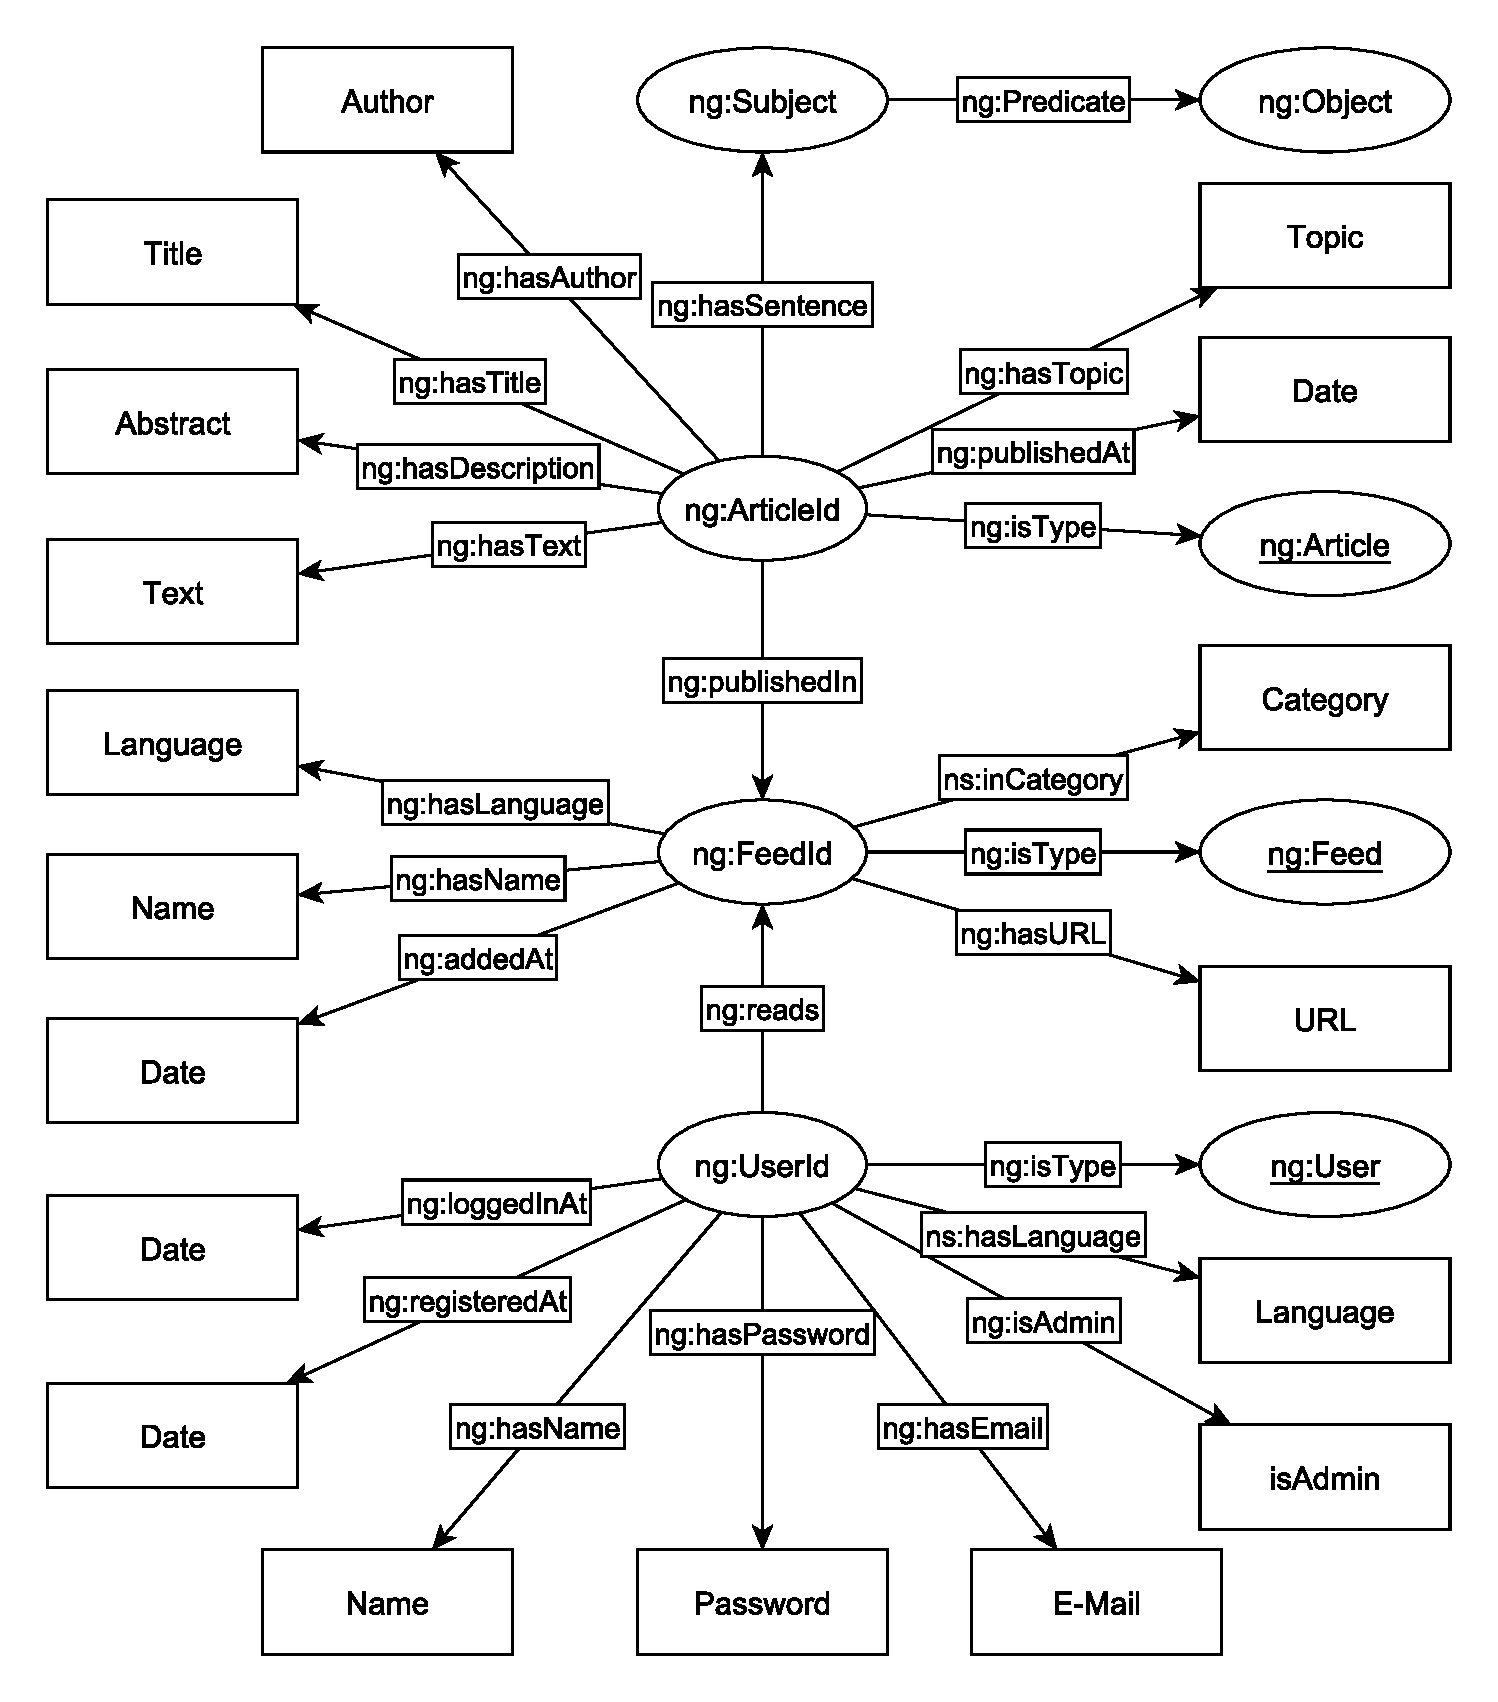
\includegraphics[width=0.90\textwidth]{Systementwurf/datenmodell/DBDiagramm.eps}
\caption{Datenbankdiagramm}
\label{fig:6.1}
\end{figure}
\section{Erläuterung}

Da wir einen Triplestore verwenden, gibt es keine wirklichen Entitäten und auch innerhalb der einzelnen Datensätze gibt es Verknüpfungen mit Kardinalität \( \neq\) 1. Die Kardinalitäten der Verknüpfungen innerhalb der Datensätze sind oben aufgeführt.

\begin{entity}{10}{User}
\begin{tabular}[ht]{|l|l|}
  \hline
  Beziehung & Kardinalität\\
  \hline
  reads & 0...n\\
  \hline
\end{tabular}
\end{entity}

\begin{entity}{20}{Artikel}
\begin{tabular}[ht]{|l|l|}
  \hline
  Beziehung & Kardinalität\\
  \hline
  publishedIn & 1\\
  \hline
  hasSentence & 0...n\\
  \hline
\end{tabular}
\end{entity}
\include{TechnischerEntwurf/07_konfiguration}
%!TEX root = ../TechnischerEntwurf.tex

\chapter{Änderungen gegenüber Fachentwurf}

Im Gegensatz zum Fachentwurf wurde nur das Datenmodell geändert. Dabei wurden die Entitäten \glqq Story\_Text\grqq , \glqq Text\_In\_Challenge \grqq~und \glqq Solve\_Task\grqq~entfernt und ihre Inhalte in anliegende Entities integriert.


%In diesem Kapitel sollt ihr Änderungen beschreiben, die gegenüber dem Fachentwurf geschehen sind.
%Es kann euch z.B. aufgefallen sein, dass ihr eine weitere Komponente benötigt, die ihr in Kapitel \ref{chap:analyse} 
%nicht in den Sequenzdiagrammen beschrieben habt. Ihr solltet dazu dann die Sequenzdiagramme anpassen 
%und hier erneut beschreiben. 
%Gleiches gilt für die Kapitel Datenmodell und Konfiguration.

%!TEX root = ../TechnischerEntwurf.tex

\chapter{Erfüllung der Kriterien}

In diesem Kapitel wird beschrieben, wie die einzelnen Kriterien, die im Pflichtenheft genannt sind, in der Software umgesetzt wurden. Dabei wird auf die Nutzung bei der Umsetzung eingegangen. Da in der Software zwei Komponenten vorhanden sind und diese dadurch sehr oft auftauchen werden, wird das Front-End nachfolgend mit seiner Bezeichnung \glqq C10\grqq~und das Back-End mit seiner Bezeichnung \glqq C10\grqq~genannt. 

\section{Musskriterien}\label{sec:musskriterien}
\must{1}{Das geforderte Minispiel wird in C10 angezeigt und die Daten dafür in C20 gespeichert}
\must{2}{Das grafisch aufbereitete Webinterface ist durch C10 komplett realisiert.}
\must{3}{Die Fenster für Aufgabenstellung und eingaben sind Teil von C10. Dabei werden die Daten für die Aufgabenstellung vom C20 angefordert und die Daten aus dem Eingabefeld werden zur Kontrolle zurück an C20 gesendet }
\must{4}{C20 besteht zum Großteil aus einer Datenbank die die anfallenden Nutzerden speichert.}
\must{5}{C20 stellt eine Benutzeroberfläche zur Verfügung, die administrative Tätigkeiten ermöglicht}
\must{6}{Die in RM5 Benutzerobfläche beinhaltet auch die Möglichkeit, Aufgaben zu erstellen.}
\must{7}{C10 bietet drei Spielmodi (Trivia-, Story und Homework-Mode).}
\must{8}{C20 hat eine Anbindung an das LDAP der Technischen Universit\"at Braunschweig.}
\must{9}{Die Game-Engine ist in C20 integriert.}


\section{Sollkriterien}\label{sec:sollkriterien}
\should{1}{Die gestellten SQL-Aufgaben haben fünf Schwierigkeitgrade.}
\should{2}{Die Gesamtsoftware ist mit leichten Leistungseinbußen auf moblien Endgeräten funktionabel.}
\should{3}{Die Software bietet verschiedene Avatare mit verschiedenen Eigenschaften die im Shop erworben werden können.}
\should{4}{Das Spielerprofil speichert verschiedene Höchstleistung des Spielers.}
\should{5}{Es werden verschiedene Ranglisten unterstützt.}


\section{Kannkriterien}\label{sec:kannkriterien}
\could{1}{Mit den entsprechenden Rechten kann jeglicher Aufgabentyp erstellt werden.}
\could{2}{Das Nutzen der Software von anderen Universitäten ist nicht vorgesehen, kann jedoch besprochen werden.}
\could{3}{Es k\"onnte ein abgespecktes Tutorial f\"ur den Trivia-Mode geben. Dies wurde nicht umgesetzt.}
\could{4}{Im Shop können, gegen Ingame-Währung, Avatare und \glqq Belt-Slots\grqq~erworben werden.} 
\could{5}{Im Minispiel erfolgen Sprünge über die Leertaste oder die linke Maustaste. Die Beltslots zum Nutzen der darin befindlichen Tränke werden mit den Tasten 1 bis 7 angewählt.}
\could{6}{Freundeslisten wird es vorerst nicht geben.}



%------Ende des Dokumentes------------------------------------------------------
\end{document}
